% Options for packages loaded elsewhere
\PassOptionsToPackage{unicode}{hyperref}
\PassOptionsToPackage{hyphens}{url}
\PassOptionsToPackage{dvipsnames,svgnames,x11names}{xcolor}
%
\documentclass[
  singlecolumn]{report}

\usepackage{amsmath,amssymb}
\usepackage{iftex}
\ifPDFTeX
  \usepackage[T1]{fontenc}
  \usepackage[utf8]{inputenc}
  \usepackage{textcomp} % provide euro and other symbols
\else % if luatex or xetex
  \usepackage{unicode-math}
  \defaultfontfeatures{Scale=MatchLowercase}
  \defaultfontfeatures[\rmfamily]{Ligatures=TeX,Scale=1}
\fi
\usepackage[]{libertinus}
\ifPDFTeX\else  
    % xetex/luatex font selection
\fi
% Use upquote if available, for straight quotes in verbatim environments
\IfFileExists{upquote.sty}{\usepackage{upquote}}{}
\IfFileExists{microtype.sty}{% use microtype if available
  \usepackage[]{microtype}
  \UseMicrotypeSet[protrusion]{basicmath} % disable protrusion for tt fonts
}{}
\makeatletter
\@ifundefined{KOMAClassName}{% if non-KOMA class
  \IfFileExists{parskip.sty}{%
    \usepackage{parskip}
  }{% else
    \setlength{\parindent}{0pt}
    \setlength{\parskip}{6pt plus 2pt minus 1pt}}
}{% if KOMA class
  \KOMAoptions{parskip=half}}
\makeatother
\usepackage{xcolor}
\usepackage[top=30mm,left=20mm,heightrounded]{geometry}
\setlength{\emergencystretch}{3em} % prevent overfull lines
\setcounter{secnumdepth}{-\maxdimen} % remove section numbering
% Make \paragraph and \subparagraph free-standing
\ifx\paragraph\undefined\else
  \let\oldparagraph\paragraph
  \renewcommand{\paragraph}[1]{\oldparagraph{#1}\mbox{}}
\fi
\ifx\subparagraph\undefined\else
  \let\oldsubparagraph\subparagraph
  \renewcommand{\subparagraph}[1]{\oldsubparagraph{#1}\mbox{}}
\fi

\usepackage{color}
\usepackage{fancyvrb}
\newcommand{\VerbBar}{|}
\newcommand{\VERB}{\Verb[commandchars=\\\{\}]}
\DefineVerbatimEnvironment{Highlighting}{Verbatim}{commandchars=\\\{\}}
% Add ',fontsize=\small' for more characters per line
\usepackage{framed}
\definecolor{shadecolor}{RGB}{241,243,245}
\newenvironment{Shaded}{\begin{snugshade}}{\end{snugshade}}
\newcommand{\AlertTok}[1]{\textcolor[rgb]{0.68,0.00,0.00}{#1}}
\newcommand{\AnnotationTok}[1]{\textcolor[rgb]{0.37,0.37,0.37}{#1}}
\newcommand{\AttributeTok}[1]{\textcolor[rgb]{0.40,0.45,0.13}{#1}}
\newcommand{\BaseNTok}[1]{\textcolor[rgb]{0.68,0.00,0.00}{#1}}
\newcommand{\BuiltInTok}[1]{\textcolor[rgb]{0.00,0.23,0.31}{#1}}
\newcommand{\CharTok}[1]{\textcolor[rgb]{0.13,0.47,0.30}{#1}}
\newcommand{\CommentTok}[1]{\textcolor[rgb]{0.37,0.37,0.37}{#1}}
\newcommand{\CommentVarTok}[1]{\textcolor[rgb]{0.37,0.37,0.37}{\textit{#1}}}
\newcommand{\ConstantTok}[1]{\textcolor[rgb]{0.56,0.35,0.01}{#1}}
\newcommand{\ControlFlowTok}[1]{\textcolor[rgb]{0.00,0.23,0.31}{#1}}
\newcommand{\DataTypeTok}[1]{\textcolor[rgb]{0.68,0.00,0.00}{#1}}
\newcommand{\DecValTok}[1]{\textcolor[rgb]{0.68,0.00,0.00}{#1}}
\newcommand{\DocumentationTok}[1]{\textcolor[rgb]{0.37,0.37,0.37}{\textit{#1}}}
\newcommand{\ErrorTok}[1]{\textcolor[rgb]{0.68,0.00,0.00}{#1}}
\newcommand{\ExtensionTok}[1]{\textcolor[rgb]{0.00,0.23,0.31}{#1}}
\newcommand{\FloatTok}[1]{\textcolor[rgb]{0.68,0.00,0.00}{#1}}
\newcommand{\FunctionTok}[1]{\textcolor[rgb]{0.28,0.35,0.67}{#1}}
\newcommand{\ImportTok}[1]{\textcolor[rgb]{0.00,0.46,0.62}{#1}}
\newcommand{\InformationTok}[1]{\textcolor[rgb]{0.37,0.37,0.37}{#1}}
\newcommand{\KeywordTok}[1]{\textcolor[rgb]{0.00,0.23,0.31}{#1}}
\newcommand{\NormalTok}[1]{\textcolor[rgb]{0.00,0.23,0.31}{#1}}
\newcommand{\OperatorTok}[1]{\textcolor[rgb]{0.37,0.37,0.37}{#1}}
\newcommand{\OtherTok}[1]{\textcolor[rgb]{0.00,0.23,0.31}{#1}}
\newcommand{\PreprocessorTok}[1]{\textcolor[rgb]{0.68,0.00,0.00}{#1}}
\newcommand{\RegionMarkerTok}[1]{\textcolor[rgb]{0.00,0.23,0.31}{#1}}
\newcommand{\SpecialCharTok}[1]{\textcolor[rgb]{0.37,0.37,0.37}{#1}}
\newcommand{\SpecialStringTok}[1]{\textcolor[rgb]{0.13,0.47,0.30}{#1}}
\newcommand{\StringTok}[1]{\textcolor[rgb]{0.13,0.47,0.30}{#1}}
\newcommand{\VariableTok}[1]{\textcolor[rgb]{0.07,0.07,0.07}{#1}}
\newcommand{\VerbatimStringTok}[1]{\textcolor[rgb]{0.13,0.47,0.30}{#1}}
\newcommand{\WarningTok}[1]{\textcolor[rgb]{0.37,0.37,0.37}{\textit{#1}}}

\providecommand{\tightlist}{%
  \setlength{\itemsep}{0pt}\setlength{\parskip}{0pt}}\usepackage{longtable,booktabs,array}
\usepackage{calc} % for calculating minipage widths
% Correct order of tables after \paragraph or \subparagraph
\usepackage{etoolbox}
\makeatletter
\patchcmd\longtable{\par}{\if@noskipsec\mbox{}\fi\par}{}{}
\makeatother
% Allow footnotes in longtable head/foot
\IfFileExists{footnotehyper.sty}{\usepackage{footnotehyper}}{\usepackage{footnote}}
\makesavenoteenv{longtable}
\usepackage{graphicx}
\makeatletter
\def\maxwidth{\ifdim\Gin@nat@width>\linewidth\linewidth\else\Gin@nat@width\fi}
\def\maxheight{\ifdim\Gin@nat@height>\textheight\textheight\else\Gin@nat@height\fi}
\makeatother
% Scale images if necessary, so that they will not overflow the page
% margins by default, and it is still possible to overwrite the defaults
% using explicit options in \includegraphics[width, height, ...]{}
\setkeys{Gin}{width=\maxwidth,height=\maxheight,keepaspectratio}
% Set default figure placement to htbp
\makeatletter
\def\fps@figure{htbp}
\makeatother
\newlength{\cslhangindent}
\setlength{\cslhangindent}{1.5em}
\newlength{\csllabelwidth}
\setlength{\csllabelwidth}{3em}
\newlength{\cslentryspacingunit} % times entry-spacing
\setlength{\cslentryspacingunit}{\parskip}
\newenvironment{CSLReferences}[2] % #1 hanging-ident, #2 entry spacing
 {% don't indent paragraphs
  \setlength{\parindent}{0pt}
  % turn on hanging indent if param 1 is 1
  \ifodd #1
  \let\oldpar\par
  \def\par{\hangindent=\cslhangindent\oldpar}
  \fi
  % set entry spacing
  \setlength{\parskip}{#2\cslentryspacingunit}
 }%
 {}
\usepackage{calc}
\newcommand{\CSLBlock}[1]{#1\hfill\break}
\newcommand{\CSLLeftMargin}[1]{\parbox[t]{\csllabelwidth}{#1}}
\newcommand{\CSLRightInline}[1]{\parbox[t]{\linewidth - \csllabelwidth}{#1}\break}
\newcommand{\CSLIndent}[1]{\hspace{\cslhangindent}#1}

\usepackage{booktabs}
\usepackage{longtable}
\usepackage{array}
\usepackage{multirow}
\usepackage{wrapfig}
\usepackage{float}
\usepackage{colortbl}
\usepackage{pdflscape}
\usepackage{tabu}
\usepackage{threeparttable}
\usepackage{threeparttablex}
\usepackage[normalem]{ulem}
\usepackage{makecell}
\usepackage{xcolor}
\usepackage{cancel}
\makeatletter
\makeatother
\makeatletter
\makeatother
\makeatletter
\@ifpackageloaded{caption}{}{\usepackage{caption}}
\AtBeginDocument{%
\ifdefined\contentsname
  \renewcommand*\contentsname{Table of contents}
\else
  \newcommand\contentsname{Table of contents}
\fi
\ifdefined\listfigurename
  \renewcommand*\listfigurename{List of Figures}
\else
  \newcommand\listfigurename{List of Figures}
\fi
\ifdefined\listtablename
  \renewcommand*\listtablename{List of Tables}
\else
  \newcommand\listtablename{List of Tables}
\fi
\ifdefined\figurename
  \renewcommand*\figurename{Figure}
\else
  \newcommand\figurename{Figure}
\fi
\ifdefined\tablename
  \renewcommand*\tablename{Table}
\else
  \newcommand\tablename{Table}
\fi
}
\@ifpackageloaded{float}{}{\usepackage{float}}
\floatstyle{ruled}
\@ifundefined{c@chapter}{\newfloat{codelisting}{h}{lop}}{\newfloat{codelisting}{h}{lop}[chapter]}
\floatname{codelisting}{Listing}
\newcommand*\listoflistings{\listof{codelisting}{List of Listings}}
\makeatother
\makeatletter
\@ifpackageloaded{caption}{}{\usepackage{caption}}
\@ifpackageloaded{subcaption}{}{\usepackage{subcaption}}
\makeatother
\makeatletter
\@ifpackageloaded{tcolorbox}{}{\usepackage[skins,breakable]{tcolorbox}}
\makeatother
\makeatletter
\@ifundefined{shadecolor}{\definecolor{shadecolor}{rgb}{.97, .97, .97}}
\makeatother
\makeatletter
\makeatother
\makeatletter
\makeatother
\ifLuaTeX
  \usepackage{selnolig}  % disable illegal ligatures
\fi
\IfFileExists{bookmark.sty}{\usepackage{bookmark}}{\usepackage{hyperref}}
\IfFileExists{xurl.sty}{\usepackage{xurl}}{} % add URL line breaks if available
\urlstyle{same} % disable monospaced font for URLs
\hypersetup{
  pdftitle={Causal effects of religious de-identification on multi-dimensional well-being},
  pdfauthor={Joseph A. Bulbulia; Don E Davis; Ken Rice; Geoffrey Troughton; Daryl Van Tongeren; Chris G. Sibley},
  pdfkeywords={Author order TBA.},
  colorlinks=true,
  linkcolor={blue},
  filecolor={Maroon},
  citecolor={Blue},
  urlcolor={Blue},
  pdfcreator={LaTeX via pandoc}}

\title{Causal effects of religious de-identification on
multi-dimensional well-being}
\usepackage{etoolbox}
\makeatletter
\providecommand{\subtitle}[1]{% add subtitle to \maketitle
  \apptocmd{\@title}{\par {\large #1 \par}}{}{}
}
\makeatother
\subtitle{An outcome-wide study}
\author{Joseph A. Bulbulia \and Don E Davis \and Ken Rice \and Geoffrey
Troughton \and Daryl Van Tongeren \and Chris G. Sibley}
\date{}

\begin{document}
\make title
\begin{abstract}
Max Weber described the loss of religion as ``the disenchantment of the
world.'' Yet, cross-sectional data fail to adequately measure the scale
of this disenchantment, if it indeed exists. Our research combines
extensive and representative national panel data with advanced causal
inference. We quantify the one-year impact of religious disaffiliation
on various facets of well-being. The most profound consequences of
religious disaffiliation are declines in charitable giving and
volunteering. Frequency of alcohol consumption increases. Disaffiliation
is causally associated with greater vengeful rumination, decreased
desire for self-control, and reduced clarity of purpose. Interestingly,
we find that an individual's sense of meaning remains constant,
irrespective of changes in religious affiliation. Across other
dimensions we find no evidence for change in average well-being. This
findings suggest future investigations into the behavioral repercussions
of religious disaffiliation on charitable behaviours. How change in
religious behaviors affect people also merits further study.
\end{abstract}
\ifdefined\Shaded\renewenvironment{Shaded}{\begin{tcolorbox}[interior hidden, enhanced, borderline west={3pt}{0pt}{shadecolor}, boxrule=0pt, frame hidden, sharp corners, breakable]}{\end{tcolorbox}}\fi

\listoffigures
\listoftables
\hypertarget{introduction}{%
\section{Introduction}\label{introduction}}

Max Weber famously described the loss of religion as ``the
disenchantment of the world''
(\protect\hyperlink{ref-wilson2014}{Wilson, J., and Sibley 2014}).
However, it is unclear whether, and in which ways, disaffiliation causes
disenchantment.

Cross-sectional data can sometimes be useful for prediction, however
they are generally ill-equipped for insights into causality. Take, for
example, a scenario where individuals with lower levels of life meaning
are observed to detach from their religious affiliations more frequently
than those reporting higher life meaning. Cross-sectional data fall
short in conclusively disentangling such complex relationships. It is
conceivable that those experiencing a sense of life's futility may
self-select out of religious institutions, resulting in a
disproportionate representation of disenchanted individuals among
non-religious groups in such surveys. Hence, if interventions were
employed to encourage these disenchanted individuals to rejoin religious
communities, they could potentially amplify feelings of life's
meaninglessness. That is, correlations can mislead us to the opposite
conclusions about true causation. Indeed the `hints' suggested in
cross-sectional data are known to strongly bias regression coefficients,
whose true causal effects may run contrary to manifest correlations
(\protect\hyperlink{ref-westreich2013}{Westreich and Greenland 2013}).
However, a persistent habit of suggesting that cross-sectional data may
`hint' at causality presents a serious challenge to psychological
science {[}J. A. Bulbulia
(\protect\hyperlink{ref-bulbulia2022}{2022}){]}(\protect\hyperlink{ref-bulbulia2021}{J.
Bulbulia et al. 2021}),

To gain clearer insights into the causal effects of religious
disaffiliation, we apply longitudinal data in this study. Our approach
aims to replicate an idealized experiment, thereby providing a more
transparent understanding of causality
(\protect\hyperlink{ref-hernuxe1n2016}{Hernán et al. 2016};
\protect\hyperlink{ref-bulbulia2022}{J. A. Bulbulia 2022};
\protect\hyperlink{ref-hernan2023}{Hernan and Robins 2023}).

\hypertarget{method}{%
\section{Method}\label{method}}

\hypertarget{sample}{%
\subsection{Sample}\label{sample}}

Data were collected as part of The New Zealand Attitudes and Values
Study (NZAVS) is an annual longitudinal national probability panel study
of social attitudes, personality, ideology and health outcomes. The
NZAVS began in 2009. It includes questionnaire responses from more than
70,000 New Zealand residents. The study includes researchers from many
New Zealand universities, including the University of Auckland, Victoria
University of Wellington, the University of Canterbury, the University
of Otago, and Waikato University. Because the survey asks the same
people to respond each year, it can track subtle change in attitudes and
values over time, and is an important resource for researchers both in
New Zealand and around the world. The NZAVS is university-based, not-
for-profit and independent of political or corporate
funding.https://doi.org/10.17605/OSF.IO/75SNB

\hypertarget{eligibility-criteria}{%
\subsection{Eligibility Criteria}\label{eligibility-criteria}}

The sample consisted of respondents to NZAVS waves Time 10, 11, and 12
(years 2018-2021) (See Appendix A.)

To emulate randomisation with our observational longitudinal data, we
selected:

\begin{enumerate}
\def\labelenumi{\arabic{enumi}.}
\tightlist
\item
  those participants who were identified as religious at the baseline
  wave (NZAVS wave 2018) and
\item
  reported a religious identification one year later.
\end{enumerate}

There were 12,600 NZAVS participants who met these criteria.

\hypertarget{the-exposure-religious-disaffiation}{%
\subsection{The Exposure: Religious
Disaffiation}\label{the-exposure-religious-disaffiation}}

As indicated in Table~\ref{tbl-transition}, of the 12600 people who were
religious at baseline, 1977 people dis-affiliated participants one year
later (NZAVS wave 2019), at the measurement year.\footnote{Cite our
  Markov paper showing that much religious change is probably
  artifactual.}

\hypertarget{tbl-transition}{}
\begin{longtable}[]{@{}ccc@{}}
\caption{\label{tbl-transition}Transition matrix}\tabularnewline
\toprule\noalign{}
From & To: stay affiliated & disaffiliate \\
\midrule\noalign{}
\endfirsthead
\toprule\noalign{}
From & To: stay affiliated & disaffiliate \\
\midrule\noalign{}
\endhead
\bottomrule\noalign{}
\endlastfoot
religious affiliate & 10623 & 1977 \\
\end{longtable}

\hypertarget{indicators-of-well-being.}{%
\subsection{Indicators of well-being.}\label{indicators-of-well-being.}}

We assessed ``disenchantment'' following Tyler J. VanderWeele, Mathur,
and Chen (\protect\hyperlink{ref-vanderweele2020}{2020}) outcome-wide
template. Outcomewide studies argue that, rather than cherry-picking one
or several domains of well-being, science may advance more rapidly, and
with greater hope for replication, by assess well-being across as many
range of indicators the data may afford. To assist with interpretation,
Tyler J. VanderWeele, Mathur, and Chen
(\protect\hyperlink{ref-vanderweele2020}{2020}) groups well-being into
larger dimensions of interest. Here, we identify five-domains: health,
embodied well-being, practical well-being, reflective well-being, and
social well-being (see Appendix A.)

\hypertarget{assumptions-for-causal-inference}{
\subsection{Assumptions for causal
inference}\label{assumptions-for-causal-inference}}

To assess a causal effect we must contrast how the world would turn out
if we were to intervene. Generally, we cannot observe individual causal
effects because for any individual case, we only observe the
intervention or its absence. We cannot both intervene and not-intervene
at once. This is called the fundamental problem of causal inference
(\protect\hyperlink{ref-rubin1976}{Rubin 1976};
\protect\hyperlink{ref-holland1986}{Holland 1986};
\protect\hyperlink{ref-bulbulia2022}{J. A. Bulbulia 2022}). Although we
cannot generally observe unit-level causal effects, it may be possible
to estimate average causal effects. We do this by contrasting the
average effect in the exposed group with the average effect in the
unexposed unexposed group. For example, average of the contrast (or
equivalently the contrast of the the averages)\footnote{Note that
  mathematically, the difference in the average expectation is
  equivalent to the average of the differences in expectation.} on the
difference scale may be expressed:

\begin{alignat*}{2}
ATE & = E[Y(1)) - E(Y(0)]\\
& = E=[Y(1) - Y(0)]
\end{alignat*}

Estimating the average treatment effects (ATE) of binary exposures or
contrasts between different exposure levels involves understanding
causal inference as counterfactual data science. The ATE is expressed
as:

   \begin{align*}
    ATE = E[Y(a) - Y(a*)]
    \end{align*}

Our causal inference is grounded on three critical assumptions:

\hypertarget{identification-assumption-1-causal-consistency}{%
\subsubsection{Identification assumption 1: Causal
consistency}\label{identification-assumption-1-causal-consistency}}

Causal consistency assumes the observed outcome aligns with the
potential outcome for a given exposure level:

\[Y^{observed} = AY(a=1) + (1-A)Y(a=0)\]

Observed outcomes can represent counterfactual outcomes under certain
exposures, such that:

\[
Y^{observed}_i = 
\begin{cases} 
Y_i(~a^*) & \text{if } A_i = a* \\
Y_i(~a~) & \text{if } A_i = a
\end{cases}
\]

Causal consistency also assumes no interference between unit treatments,
allowing potential outcomes to be set to the observed outcomes. For this
assumption to hold, we require ``treatment variation irrelevance.'' If
there are (1) well-defined outcomes for each treatment version, and (2)
no confounding effects, the multiple versions of treatments can be used
to estimate the causal effect:

\[K \coprod Y(k) | L\] or equivalently \[Y(k) \coprod K | L\]

Here, the treatment \(A\) is essentially a function of \(K\) treatments,
\(A = f(k_1...k_v)\) versions

Limitations exist, however, when interventions are ill-defined, or the
causal effect's interpretation is ambiguous. Put simply, given there are
unknown ways of becoming religiously disaffiliated the interpretation of
``disaffiliation'' may be strained. It is strained in the sense that we
would not know how to intervene to \emph{make} a religiously affiliated
person disaffiliate. We will return to this question in the discussion.

\hypertarget{identification-assumption-2-exchangability}{%
\subsubsection{Identification assumption 2:
Exchangability}\label{identification-assumption-2-exchangability}}

Exchangability assumes treatment assignment is independent of potential
outcomes, given observed covariates. This is the ``no-confounding''
assumption that many psychologists have learned in association with
experimental design. In the setting of observational data, we emulate
randomisation by conditioning on indicators that may lead to an
association of the exposure \(A\) and the outcome \(Y\) in the absence
of causation.

\[Y(a)\coprod  A|L\] or \[A \coprod  Y(a)|L\]

Where exchangability holds, we calculate the Average Treatment Effect
(ATE)

\[
ATE = E[Y(a*)|L = l] - E[Y(a)|L = l] 
\]

Put differently, conditioning on confounders ensures \emph{balance} in
their distribution across exposures.

\hypertarget{identification-assumption-3-positivity}{%
\subsubsection{Identification assumption 3:
Positivity}\label{identification-assumption-3-positivity}}

Positivity is satisfied if there is a positive probability of receiving
or not receiving exposure at all covariate levels. Expressed as:

\begin{equation}
0 < \Pr(A=a|L)<1, ~ \forall a \in A, ~ \forall a \in L
\end{equation}

There are two types of positivity violation.

\begin{itemize}
\item
  \textbf{Random non-positivity}: Occurs when the causal effect of a
  missing observation is presumed to exist. This violation is the only
  one verifiable by data. Here, we check and report it.
\item
  \textbf{Deterministic non-positivity}: Occurs when the causal effect
  is inconceivable. For example, the causal effect of hysterectomy in
  biological males violates deterministic non-positivity.
\end{itemize}

\hypertarget{causal-identification-strategy}{%
\subsection{Causal identification
Strategy}\label{causal-identification-strategy}}

Effects must follow causes. To avoid the problems of reverse causation,
we measured outcomes during the year following the exposure (NZAVS wave
2020). The causal graph presented in Figure~\ref{fig-outcomewide-dag}
describes our method for confouding control. We follow Tyler J.
VanderWeele, Mathur, and Chen
(\protect\hyperlink{ref-vanderweele2020}{2020}) in adopting a modified
disjunctive cause criterion whisch states:

\begin{enumerate}
\def\labelenumi{\arabic{enumi}.}
\item
  \textbf{Identify all relevant factors}: first, find every covariates
  that can influence either the exposure (disaffiliation) or the
  outcomes (across the five domains), or both. These factors are any
  variable that can have an impact on the exposure or outcome, are that
  might be the effect of such a factor.
\item
  \textbf{Remove instrumental variables}: next, take out any factors
  that are known to be `instrumental variables'. These are factors that
  cause the exposure but do not affect the outcome. Including
  instrumental variables reduces efficiency.
\item
  \textbf{Include proxy variables for unmeasured common causes}: if
  there are any unmeasured factors that influence both the exposure and
  outcome, but we don not have direct measurements for them, we should
  try to include a proxy for these. A proxy is an effect of the
  variable.
\item
  \textbf{Control for prior exposure}: Controlling for prior exposure
  assesses the effects of ``incident exposure'' rather than ``prevalent
  exposure'' - and is a critical step in causal
  inference(\protect\hyperlink{ref-danaei2012}{Danaei, Tavakkoli, and
  Hernán 2012}; \protect\hyperlink{ref-hernan2023}{Hernan and Robins
  2023}). By including prior exposure in the analysis, we can more
  effectively emulate a controlled trial. This approach not only helps
  interpret the effect of exposure changes but also strengthens
  confounding control. It aids in avoiding reverse causation and
  managing other forms of unmeasured confounding. This setup ensures
  that any unmeasured confounder would have to influence both the
  outcome and initial exposure, irrespective of previous exposure
  levels, to explain an observed exposure-outcome association.
\item
  \textbf{Control for prior outcome}: It is also vital to control for
  the outcome measured at baseline -- the `baseline outcome'. This
  tactic aims to rule out reverse causation by ensuring that the
  cause-effect relationship follows the right temporal order. Even
  though it does not eliminate the possibility of reverse causation,
  controlling for the baseline outcome helps mitigate its effects.
  Hence, along with a rich set of covariates, the baseline outcome
  should be included in the covariate set to make the confounding
  control assumption as plausible as possible. It is often the strongest
  confounder affecting both the exposure and subsequent outcome. (For a
  detailed account of confounding control in three-wave panel designs
  see Tyler J. VanderWeele, Mathur, and Chen
  (\protect\hyperlink{ref-vanderweele2020}{2020}))
\end{enumerate}

To avoid bias, we must also handle missing data arising from
non-response or panel attrition (loss-to-follow up). Selection bias
occurs when\ldots{} To address selection bias we perform multiple
imputation \emph{separately} by each exposure condition, and combine the
imputations after modelling missingness conditional on the observed
covariates (see: (\protect\hyperlink{ref-zhang2023}{Zhang et al. 2023};
\protect\hyperlink{ref-westreich2015}{Westreich et al. 2015})) . We
implement multiple imputation using the \texttt{mice} package in R
(\protect\hyperlink{ref-vanbuuren2018}{Van Buuren 2018}). We imputed 10
x missing data sets which were passed separately to the the
\texttt{MatchThem} and \texttt{WeightIt} packages for propensity score
matching. There are several ways in which selection bias can occur from
missing responses and loss to follow up (see
(\protect\hyperlink{ref-hernuxe1n2016}{Hernán et al. 2016};
\protect\hyperlink{ref-hernan2023}{Hernan and Robins 2023}),
Figure~\ref{fig-outcomewide-dag} presents a scenario in which the
exposure \(A\) affects the process of selection. For example \ldots{}
(say more).

\begin{figure}

%{\centering \includegraphics[width=0.8\textwidth,height=\textheight]{target-trial-religion-loss_files/figure-pdf/fig-outcomewide-dag-1.pdf}

}

\caption{\label{fig-outcomewide-dag}Causal graph: three-wave panel
design with selection bias}

\end{figure}

\hypertarget{causal-estimation}{%
\subsection{Causal estimation}\label{causal-estimation}}

To obtain causal contrasts we use doubly robust methods. These combine
inverse probability of treatment weights (propensity scores) with
regression stratification. There are two models at work in a doubly
robust estimator.

We use a Doubly Robust Estimation method, which effectively combines the
strengths of the IPTW and G-computation methods (see:
\href{https://go-bayes.github.io/psych-434-2023/content/09-content.html\#comprehensive-checklist-for-detailed-reporting-of-a-causal-inferenctial-study-e.g.-assessment-3-option-2}{here}.
The technique utilises both the propensity score and the outcome model,
making it ``doubly robust.'' This implies that if either of these models
is correctly specified, the estimation will not be biased.

\textbf{Step 1} The first step is to estimate the propensity score. The
propensity score, denoted as \(e(L)\), is the conditional probability of
the exposure \(A = 1\) given the covariates \(L\). The appropriate model
to estimate this can be chosen based on the nature of the data and the
exposure.

\[e = P(A = 1 | L) = f_A(L; \theta_A)\]

In this equation, \(f_A(L; \theta_A)\) is a function that estimates the
probability of the exposure \(A = 1\) given covariates \(L\). Here, we
use the \texttt{ebalance} method from the \texttt{clarify} package,
which we have found to ensure good balance on the confounders (see fig
below). We then calculate the weights for each individual, denoted as
\(v\), using the estimated propensity score:

\[
v = 
\begin{cases} 
\frac{1}{e} & \text{if } A = 1 \\
\frac{1}{1-e} & \text{if } A = 0 
\end{cases}
\]

Here, \(v\) depends on \(A\), and is calculated as the inverse of the
propensity score for exposed individuals and as the inverse of \(1-e\)
for unexposed individuals.

\textbf{Step 2} The next step involves fitting a weighted outcome model.
Using the weights computed from the estimated propensity scores, a model
for the outcome \(Y\), conditional on the exposure \(A\), is fitted.

\[ \hat{E}(Y|A, L; V) = f_Y(A, L ; \theta_Y, V) \]

In this model, \(f_Y\) is a function (in our case a weighted regression
model) with parameters \(θ_Y\). The weights \(V\) are incorporated into
the estimation process, affecting the contribution of each observation
to the estimation of \(θ_Y\), but they are not an additional variable in
the model. Additionally, following {``Agnostic Notes on Regression
Adjustments to Experimental Data: Reexamining Freedman{'}s Critique''}
(\protect\hyperlink{ref-agnostic}{n.d.}), we take the interaction of the
exposure and baseline covariates when estimating our regression model.
For binary outcomes we model the rate ratio using Poisson regression.
Although binomial regression is acceptable when the outcome is rare
(less than 10\%), non-collapsability leads means that we cannot
interpret results as marginal causal effects. For consistency we use the
Poisson model with robust standard errors.

\textbf{Step 3} The third step is to simulate the potential outcome for
each individual under the hypothetical scenario where everyone is
exposed to the intervention \(A=a\), irrespective of their actual
exposure level:

\[\hat{E}(a) = \hat{E}[Y_i|A=a; L,\hat{\theta}_Y, v_i]\]

This expectation is calculated for each individual \(i\), with
individual-specific weights \(v_i\).

\textbf{Step 4} Finally, we estimate the average causal effect. We
compute the estimated expected value of the potential outcomes under
each intervention level:

\[\hat{\delta} = \hat{E}[Y(a)] - \hat{E}[Y(a')]\]

The difference \(\delta\) represents the average causal effect of
changing the exposure from level \(a'\) to level \(a\).

For standard errors and confidence intervals, we use simulation-based
inference methods (\protect\hyperlink{ref-greifer2023}{Greifer et al.
2023}).

\hypertarget{baseline-confounders-exposure-and-outcome-measures}{%
\subsection{Baseline confounders, exposure, and outcome
measures}\label{baseline-confounders-exposure-and-outcome-measures}}

( \emph{Say more.} \emph{Tables here} )

((\emph{Insert section on why the assumptions of factor models are much
stronger than people are aware, and that -- despite a loss of efficiency
-- it is often best to use single item measures except when there are
clear} conceptual* reasons to do otherwise.* ))

\textbf{SEE}: (\protect\hyperlink{ref-vanderweele2022}{Tyler J.
VanderWeele 2022})

\hypertarget{results}{%
\section{Results}\label{results}}

\hypertarget{effects-on-health}{%
\subsection{Effects on health}\label{effects-on-health}}

As indicate in Figure~\ref{fig-results-health}, the expected + one-year
effect of religious disaffiliation does not reliably affect health as
subjectively reported across NZAVS domains. However, we find that
disaffilation is causally associated with increases in both the average
intensity and frequency of alcohol consumption.

It has long been known that alcohol consumption can have damaging health
and social effects. However, it is unclear whether the changes we detect
here translate to other domains.

\begin{figure}

{\centering 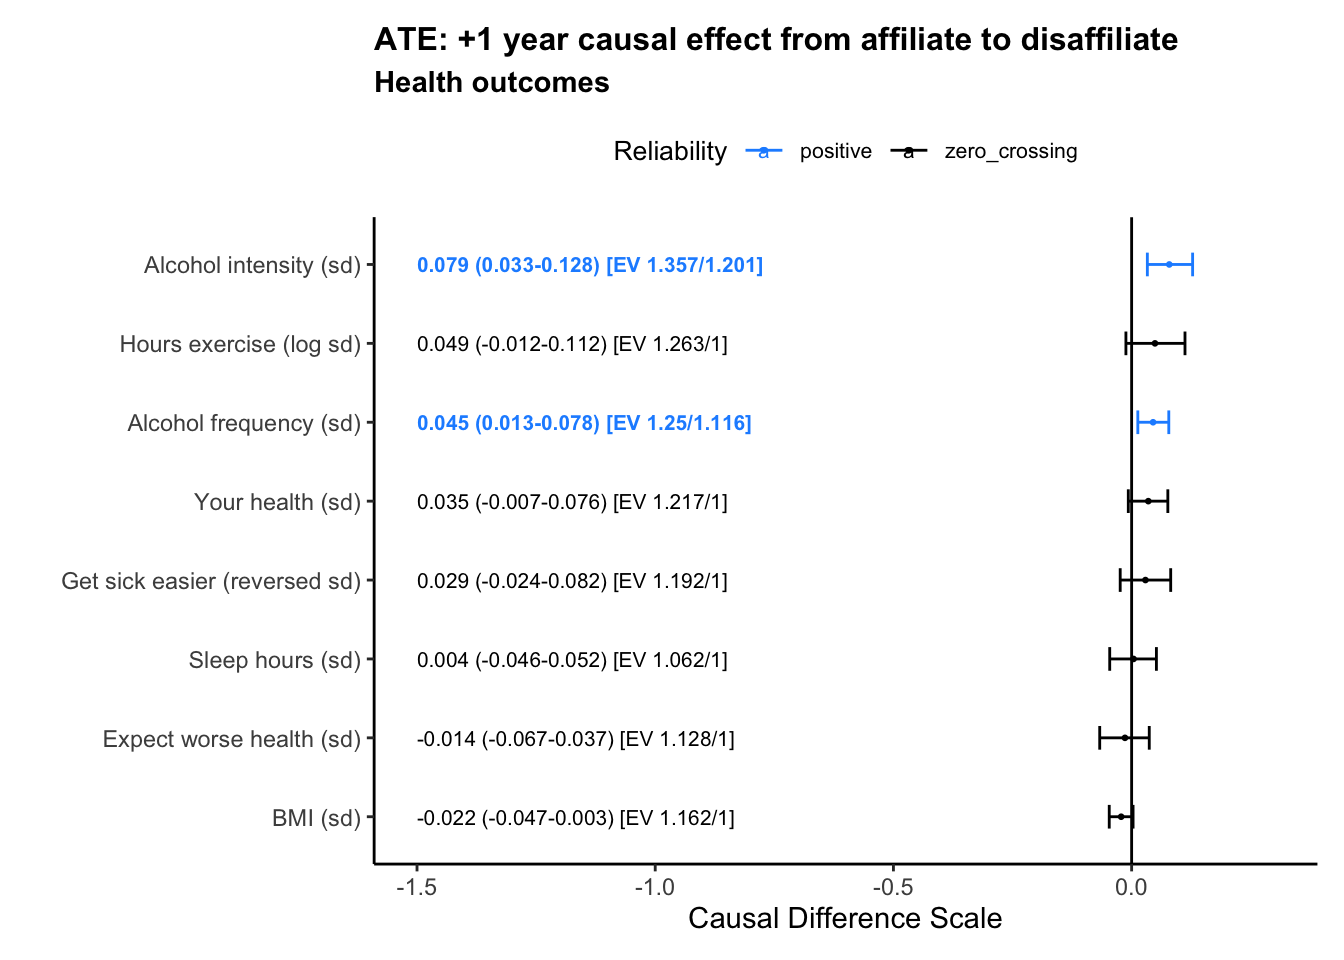
\includegraphics{target-trial-religion-loss_files/figure-pdf/fig-results-health-1.pdf}

}

\caption{\label{fig-results-health}Causal effects of religious loss on
reported physical health}

\end{figure}

\hypertarget{tbl-results-health}{}
\begin{longtable}[]{@{}
  >{\raggedright\arraybackslash}p{(\columnwidth - 10\tabcolsep) * \real{0.3704}}
  >{\raggedleft\arraybackslash}p{(\columnwidth - 10\tabcolsep) * \real{0.1975}}
  >{\raggedleft\arraybackslash}p{(\columnwidth - 10\tabcolsep) * \real{0.0988}}
  >{\raggedleft\arraybackslash}p{(\columnwidth - 10\tabcolsep) * \real{0.0864}}
  >{\raggedleft\arraybackslash}p{(\columnwidth - 10\tabcolsep) * \real{0.0988}}
  >{\raggedleft\arraybackslash}p{(\columnwidth - 10\tabcolsep) * \real{0.1481}}@{}}
\caption{\label{tbl-results-health}Table of results for the health
domain}\tabularnewline
\toprule\noalign{}
\begin{minipage}[b]{\linewidth}\raggedright
\end{minipage} & \begin{minipage}[b]{\linewidth}\raggedleft
E{[}Y(1){]}-E{[}Y(0){]}
\end{minipage} & \begin{minipage}[b]{\linewidth}\raggedleft
2.5 \%
\end{minipage} & \begin{minipage}[b]{\linewidth}\raggedleft
97.5 \%
\end{minipage} & \begin{minipage}[b]{\linewidth}\raggedleft
E\_Value
\end{minipage} & \begin{minipage}[b]{\linewidth}\raggedleft
E\_Val\_bound
\end{minipage} \\
\midrule\noalign{}
\endfirsthead
\toprule\noalign{}
\begin{minipage}[b]{\linewidth}\raggedright
\end{minipage} & \begin{minipage}[b]{\linewidth}\raggedleft
E{[}Y(1){]}-E{[}Y(0){]}
\end{minipage} & \begin{minipage}[b]{\linewidth}\raggedleft
2.5 \%
\end{minipage} & \begin{minipage}[b]{\linewidth}\raggedleft
97.5 \%
\end{minipage} & \begin{minipage}[b]{\linewidth}\raggedleft
E\_Value
\end{minipage} & \begin{minipage}[b]{\linewidth}\raggedleft
E\_Val\_bound
\end{minipage} \\
\midrule\noalign{}
\endhead
\bottomrule\noalign{}
\endlastfoot
BMI (sd) & -0.0216 & -0.0471 & 0.0033 & 1.162 & 1.000 \\
Alcohol frequency (sd) & 0.0448 & 0.0125 & 0.0782 & 1.250 & 1.116 \\
Alcohol intensity (sd) & 0.0788 & 0.0327 & 0.1281 & 1.357 & 1.201 \\
Hours exercise (log sd) & 0.0487 & -0.0123 & 0.1124 & 1.263 & 1.000 \\
Your health (sd) & 0.0355 & -0.0074 & 0.0764 & 1.217 & 1.000 \\
Get sick easier (reversed sd) & 0.0289 & -0.0243 & 0.0821 & 1.192 &
1.000 \\
Expect worse health (sd) & -0.0143 & -0.0673 & 0.0366 & 1.128 & 1.000 \\
Sleep hours (sd) & 0.0037 & -0.0465 & 0.0525 & 1.062 & 1.000 \\
\end{longtable}

Table~\ref{tbl-results-health} presents the Population Average Treatment
Effect (PATE) represents the expected difference in outcomes between
treatment and control groups for the New Zealand population. We observed
the following:

For the outcome `Alcohol intensity (sd)', the PATE causal contrast is
0.079. The confidence interval ranges from 0.033 to 0.128. The E-value
for this outcome is 1.357, indicating reliable evidence for causality.

For the outcome `Hours exercise (log sd)', the PATE causal contrast is
0.049. The confidence interval ranges from -0.012 to 0.112. The E-value
for this outcome confirms the causal contrast is unreliable.

For the outcome `Alcohol frequency (sd)', the PATE causal contrast is
0.045. The confidence interval ranges from 0.013 to 0.078. The E-value
for this outcome is 1.25, indicating reliable evidence for causality.

For the outcome `Your health (sd)', the PATE causal contrast is 0.035.
The confidence interval ranges from -0.007 to 0.076. The E-value for
this outcome confirms the causal contrast is unreliable.

For the outcome `Get sick easier (reversed sd)', the PATE causal
contrast is 0.029. The confidence interval ranges from -0.024 to 0.082.
The E-value for this outcome confirms the causal contrast is unreliable.

For the outcome `Sleep hours (sd)', the PATE causal contrast is 0.004.
The confidence interval ranges from -0.046 to 0.052. The E-value for
this outcome confirms the causal contrast is unreliable.

For the outcome `Expect worse health (sd)', the PATE causal contrast is
-0.014. The confidence interval ranges from -0.067 to 0.037. The E-value
for this outcome confirms the causal contrast is unreliable.

For the outcome `BMI (sd)', the PATE causal contrast is -0.022. The
confidence interval ranges from -0.047 to 0.003. The E-value for this
outcome confirms the causal contrast is unreliable.

\begin{figure}

{\centering 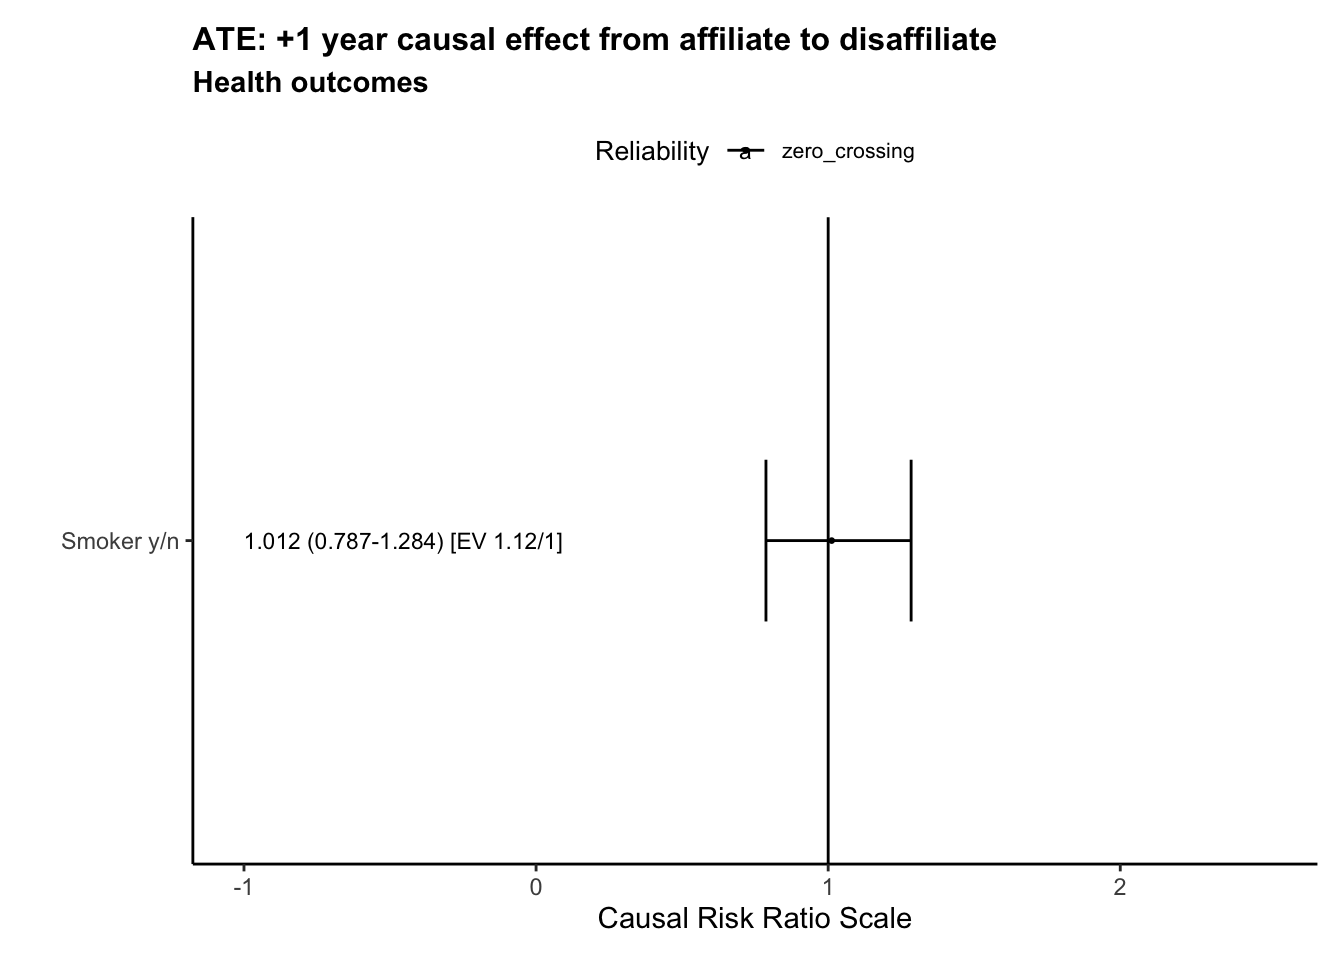
\includegraphics{target-trial-religion-loss_files/figure-pdf/fig-results-health-rr-1.pdf}

}

\caption{\label{fig-results-health-rr}Causal effects of religious loss
on smoking (risk ratio)}

\end{figure}

\hypertarget{tbl-results-health-rr}{}
\begin{longtable}[]{@{}lrrrrr@{}}
\caption{\label{tbl-results-health-rr}Table of results for
smoking}\tabularnewline
\toprule\noalign{}
& E{[}Y(1){]}/E{[}Y(0){]} & 2.5 \% & 97.5 \% & E\_Value &
E\_Val\_bound \\
\midrule\noalign{}
\endfirsthead
\toprule\noalign{}
& E{[}Y(1){]}/E{[}Y(0){]} & 2.5 \% & 97.5 \% & E\_Value &
E\_Val\_bound \\
\midrule\noalign{}
\endhead
\bottomrule\noalign{}
\endlastfoot
Smoker y/n & 1.0116 & 0.7867 & 1.2838 & 1.12 & 1 \\
\end{longtable}

For the outcome `Smoker y/n', the PATE causal contrast is 1.012. The
confidence interval ranges from 0.787 to 1.284. The E-value for this
outcome confirms the causal contrast unreliable.

\hypertarget{effects-on-embodied-well-being}{%
\subsection{Effects on embodied
well-being}\label{effects-on-embodied-well-being}}

\begin{figure}

{\centering 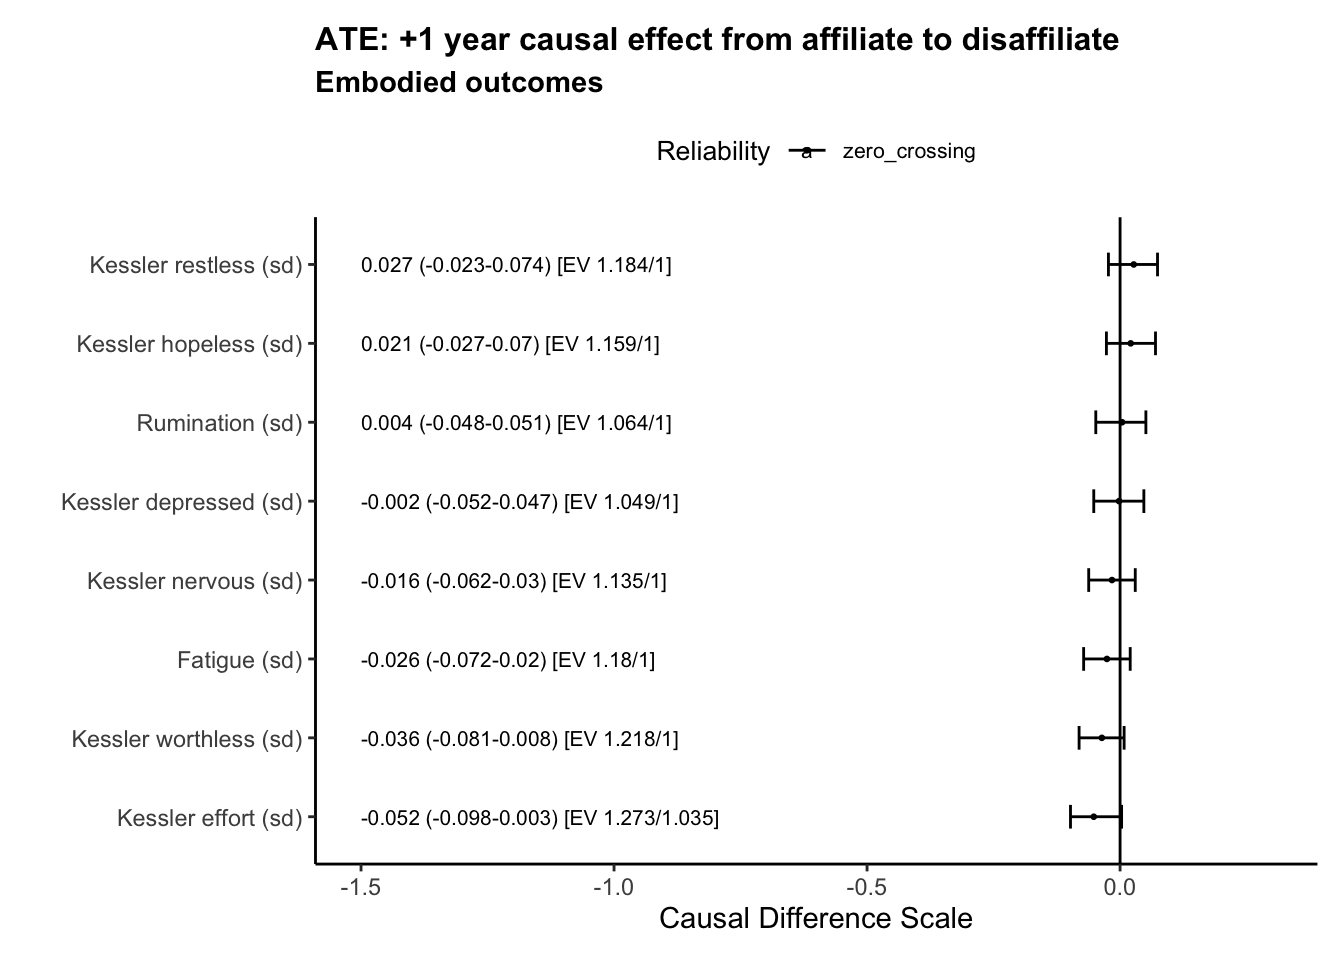
\includegraphics{target-trial-religion-loss_files/figure-pdf/fig-results-embodied-1.pdf}

}

\caption{\label{fig-results-embodied}Causal effects of religious loss on
embodied well-being}

\end{figure}

\hypertarget{tbl-results-embodied}{}
\begin{longtable}[]{@{}
  >{\raggedright\arraybackslash}p{(\columnwidth - 10\tabcolsep) * \real{0.3108}}
  >{\raggedleft\arraybackslash}p{(\columnwidth - 10\tabcolsep) * \real{0.2162}}
  >{\raggedleft\arraybackslash}p{(\columnwidth - 10\tabcolsep) * \real{0.1081}}
  >{\raggedleft\arraybackslash}p{(\columnwidth - 10\tabcolsep) * \real{0.0946}}
  >{\raggedleft\arraybackslash}p{(\columnwidth - 10\tabcolsep) * \real{0.1081}}
  >{\raggedleft\arraybackslash}p{(\columnwidth - 10\tabcolsep) * \real{0.1622}}@{}}
\caption{\label{tbl-results-embodied}Table of results for the embodied
well-being domain}\tabularnewline
\toprule\noalign{}
\begin{minipage}[b]{\linewidth}\raggedright
\end{minipage} & \begin{minipage}[b]{\linewidth}\raggedleft
E{[}Y(1){]}-E{[}Y(0){]}
\end{minipage} & \begin{minipage}[b]{\linewidth}\raggedleft
2.5 \%
\end{minipage} & \begin{minipage}[b]{\linewidth}\raggedleft
97.5 \%
\end{minipage} & \begin{minipage}[b]{\linewidth}\raggedleft
E\_Value
\end{minipage} & \begin{minipage}[b]{\linewidth}\raggedleft
E\_Val\_bound
\end{minipage} \\
\midrule\noalign{}
\endfirsthead
\toprule\noalign{}
\begin{minipage}[b]{\linewidth}\raggedright
\end{minipage} & \begin{minipage}[b]{\linewidth}\raggedleft
E{[}Y(1){]}-E{[}Y(0){]}
\end{minipage} & \begin{minipage}[b]{\linewidth}\raggedleft
2.5 \%
\end{minipage} & \begin{minipage}[b]{\linewidth}\raggedleft
97.5 \%
\end{minipage} & \begin{minipage}[b]{\linewidth}\raggedleft
E\_Value
\end{minipage} & \begin{minipage}[b]{\linewidth}\raggedleft
E\_Val\_bound
\end{minipage} \\
\midrule\noalign{}
\endhead
\bottomrule\noalign{}
\endlastfoot
Fatigue (sd) & -0.0259 & -0.0717 & 0.0200 & 1.180 & 1.000 \\
Rumination (sd) & 0.0040 & -0.0479 & 0.0513 & 1.064 & 1.000 \\
Kessler depressed (sd) & -0.0024 & -0.0520 & 0.0472 & 1.049 & 1.000 \\
Kessler effort (sd) & -0.0516 & -0.0982 & 0.0027 & 1.273 & 1.035 \\
Kessler hopeless (sd) & 0.0208 & -0.0267 & 0.0695 & 1.159 & 1.000 \\
Kessler nervous (sd) & -0.0157 & -0.0620 & 0.0296 & 1.135 & 1.000 \\
Kessler restless (sd) & 0.0268 & -0.0228 & 0.0740 & 1.184 & 1.000 \\
Kessler worthless (sd) & -0.0357 & -0.0808 & 0.0084 & 1.218 & 1.000 \\
\end{longtable}

Table~\ref{tbl-results-embodied} presents the Population Average
Treatment Effect (PATE) for the embodied domain.

For the outcome `Kessler restless (sd)', the PATE causal contrast is
0.027. The confidence interval ranges from -0.023 to 0.074. The E-value
for this outcome confirms the causal contrast is unreliable.

For the outcome `Kessler hopeless (sd)', the PATE causal contrast is
0.021. The confidence interval ranges from -0.027 to 0.07. The E-value
for this outcome confirms the causal contrast is unreliable.

For the outcome `Rumination (sd)', the PATE causal contrast is 0.004.
The confidence interval ranges from -0.048 to 0.051. The E-value for
this outcome confirms the causal contrast is unreliable.

For the outcome `Kessler depressed (sd)', the PATE causal contrast is
-0.002. The confidence interval ranges from -0.052 to 0.047. The E-value
for this outcome confirms the causal contrast is unreliable.

For the outcome `Kessler nervous (sd)', the PATE causal contrast is
-0.016. The confidence interval ranges from -0.062 to 0.03. The E-value
for this outcome confirms the causal contrast is unreliable.

For the outcome `Fatigue (sd)', the PATE causal contrast is -0.026. The
confidence interval ranges from -0.072 to 0.02. The E-value for this
outcome confirms the causal contrast is unreliable.

For the outcome `Kessler worthless (sd)', the PATE causal contrast is
-0.036. The confidence interval ranges from -0.081 to 0.008. The E-value
for this outcome confirms the causal contrast is unreliable.

For the outcome `Kessler effort (sd)', the PATE causal contrast is
-0.052. The confidence interval ranges from -0.098 to 0.003. The E-value
for this outcome confirms the causal contrast is unreliable.

\hypertarget{effects-on-practical-well-being}{%
\subsection{Effects on practical
well-being}\label{effects-on-practical-well-being}}

\begin{figure}

{\centering 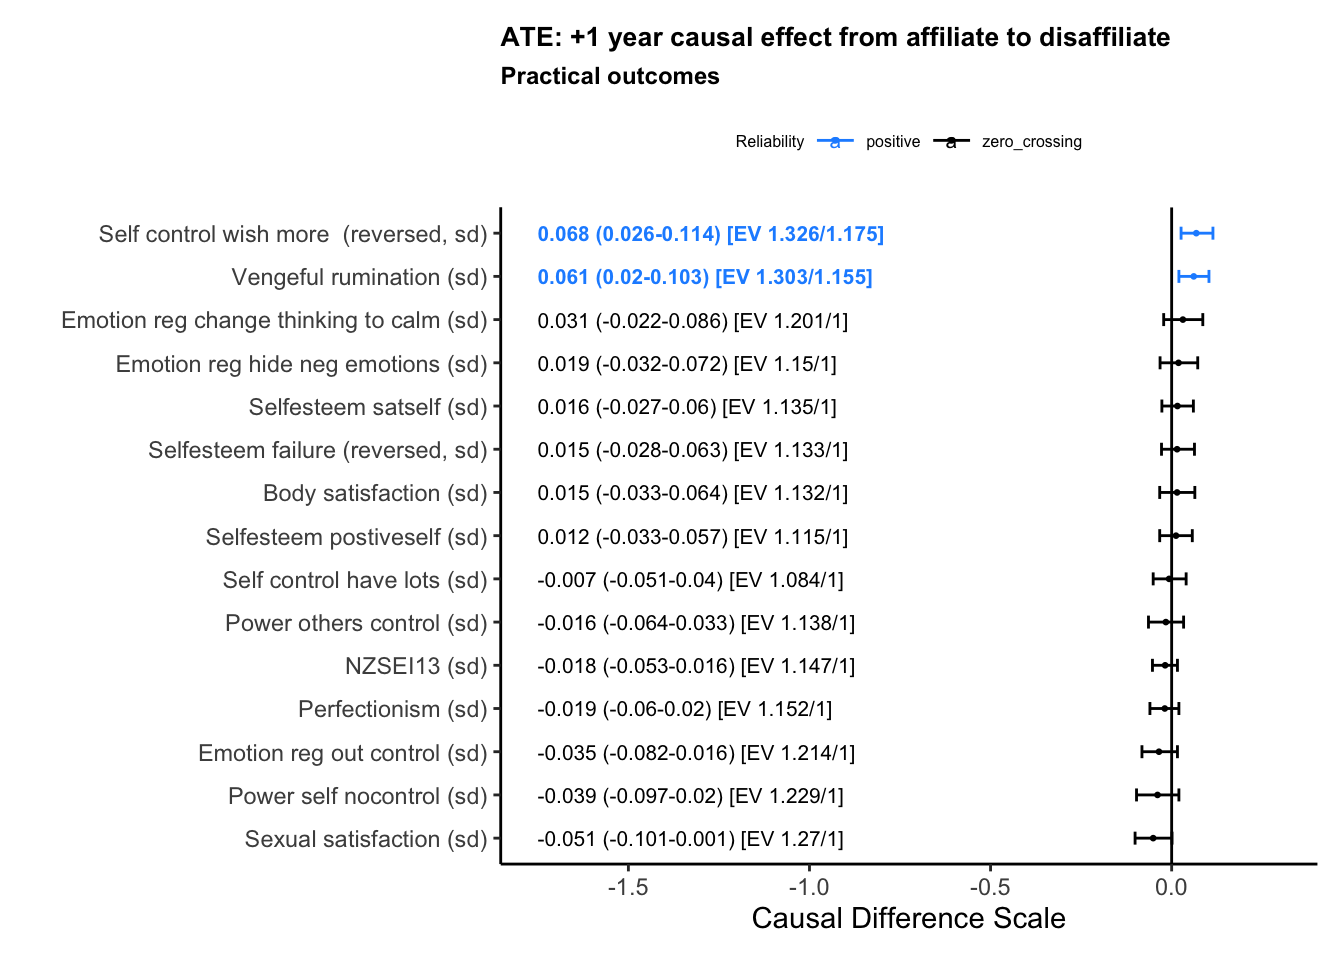
\includegraphics{target-trial-religion-loss_files/figure-pdf/fig-results-practical-well-being-1.pdf}

}

\caption{\label{fig-results-practical-well-being}Causal effects of
religious loss on practical well-being}

\end{figure}

\hypertarget{tbl-results-practical}{}
\begin{longtable}[]{@{}
  >{\raggedright\arraybackslash}p{(\columnwidth - 10\tabcolsep) * \real{0.4457}}
  >{\raggedleft\arraybackslash}p{(\columnwidth - 10\tabcolsep) * \real{0.1739}}
  >{\raggedleft\arraybackslash}p{(\columnwidth - 10\tabcolsep) * \real{0.0870}}
  >{\raggedleft\arraybackslash}p{(\columnwidth - 10\tabcolsep) * \real{0.0761}}
  >{\raggedleft\arraybackslash}p{(\columnwidth - 10\tabcolsep) * \real{0.0870}}
  >{\raggedleft\arraybackslash}p{(\columnwidth - 10\tabcolsep) * \real{0.1304}}@{}}
\caption{\label{tbl-results-practical}Table of results for the practical
well-being domain}\tabularnewline
\toprule\noalign{}
\begin{minipage}[b]{\linewidth}\raggedright
\end{minipage} & \begin{minipage}[b]{\linewidth}\raggedleft
E{[}Y(1){]}-E{[}Y(0){]}
\end{minipage} & \begin{minipage}[b]{\linewidth}\raggedleft
2.5 \%
\end{minipage} & \begin{minipage}[b]{\linewidth}\raggedleft
97.5 \%
\end{minipage} & \begin{minipage}[b]{\linewidth}\raggedleft
E\_Value
\end{minipage} & \begin{minipage}[b]{\linewidth}\raggedleft
E\_Val\_bound
\end{minipage} \\
\midrule\noalign{}
\endfirsthead
\toprule\noalign{}
\begin{minipage}[b]{\linewidth}\raggedright
\end{minipage} & \begin{minipage}[b]{\linewidth}\raggedleft
E{[}Y(1){]}-E{[}Y(0){]}
\end{minipage} & \begin{minipage}[b]{\linewidth}\raggedleft
2.5 \%
\end{minipage} & \begin{minipage}[b]{\linewidth}\raggedleft
97.5 \%
\end{minipage} & \begin{minipage}[b]{\linewidth}\raggedleft
E\_Value
\end{minipage} & \begin{minipage}[b]{\linewidth}\raggedleft
E\_Val\_bound
\end{minipage} \\
\midrule\noalign{}
\endhead
\bottomrule\noalign{}
\endlastfoot
Sexual satisfaction (sd) & -0.0507 & -0.1008 & 0.0009 & 1.270 & 1.000 \\
Perfectionism (sd) & -0.0194 & -0.0601 & 0.0201 & 1.152 & 1.000 \\
Body satisfaction (sd) & 0.0151 & -0.0332 & 0.0642 & 1.132 & 1.000 \\
Vengeful rumination (sd) & 0.0612 & 0.0203 & 0.1028 & 1.303 & 1.155 \\
Power self nocontrol (sd) & -0.0387 & -0.0966 & 0.0203 & 1.229 &
1.000 \\
Power others control (sd) & -0.0163 & -0.0644 & 0.0329 & 1.138 &
1.000 \\
Selfesteem satself (sd) & 0.0157 & -0.0271 & 0.0604 & 1.135 & 1.000 \\
Selfesteem postiveself (sd) & 0.0118 & -0.0328 & 0.0569 & 1.115 &
1.000 \\
Selfesteem failure (reversed, sd) & 0.0152 & -0.0280 & 0.0626 & 1.133 &
1.000 \\
Self control have lots (sd) & -0.0066 & -0.0513 & 0.0397 & 1.084 &
1.000 \\
Self control wish more (reversed, sd) & 0.0684 & 0.0258 & 0.1135 & 1.326
& 1.175 \\
Emotion reg out control (sd) & -0.0347 & -0.0817 & 0.0155 & 1.214 &
1.000 \\
Emotion reg hide neg emotions (sd) & 0.0189 & -0.0315 & 0.0719 & 1.150 &
1.000 \\
Emotion reg change thinking to calm (sd) & 0.0312 & -0.0217 & 0.0863 &
1.201 & 1.000 \\
NZSEI13 (sd) & -0.0183 & -0.0531 & 0.0161 & 1.147 & 1.000 \\
\end{longtable}

Table~\ref{tbl-results-practical} presents the Population Average
Treatment Effect (PATE) for the practical well-being domain.

For the outcome `Self control wish more (reversed, sd)', the PATE causal
contrast is 0.068. The confidence interval ranges from 0.026 to 0.114.
The E-value for this outcome is 1.326, indicating reliable evidence for
causality.

For the outcome `Vengeful rumination (sd)', the PATE causal contrast is
0.061. The confidence interval ranges from 0.02 to 0.103. The E-value
for this outcome is 1.303, indicating reliable evidence for causality.

For the outcome `Emotion reg change thinking to calm (sd)', the PATE
causal contrast is 0.031. The confidence interval ranges from -0.022 to
0.086. The E-value for this outcome confirms the causal contrast is
unreliable.

For the outcome `Emotion reg hide neg emotions (sd)', the PATE causal
contrast is 0.019. The confidence interval ranges from -0.032 to 0.072.
The E-value for this outcome confirms the causal contrast is unreliable.

For the outcome `Selfesteem satself (sd)', the PATE causal contrast is
0.016. The confidence interval ranges from -0.027 to 0.06. The E-value
for this outcome confirms the causal contrast is unreliable.

For the outcome `Selfesteem failure (reversed, sd)', the PATE causal
contrast is 0.015. The confidence interval ranges from -0.028 to 0.063.
The E-value for this outcome confirms the causal contrast is unreliable.

For the outcome `Body satisfaction (sd)', the PATE causal contrast is
0.015. The confidence interval ranges from -0.033 to 0.064. The E-value
for this outcome confirms the causal contrast is unreliable.

For the outcome `Selfesteem postiveself (sd)', the PATE causal contrast
is 0.012. The confidence interval ranges from -0.033 to 0.057. The
E-value for this outcome confirms the causal contrast is unreliable.

For the outcome `Self control have lots (sd)', the PATE causal contrast
is -0.007. The confidence interval ranges from -0.051 to 0.04. The
E-value for this outcome confirms the causal contrast is unreliable.

For the outcome `Power others control (sd)', the PATE causal contrast is
-0.016. The confidence interval ranges from -0.064 to 0.033. The E-value
for this outcome confirms the causal contrast is unreliable.

For the outcome `NZSEI13 (sd)', the PATE causal contrast is -0.018. The
confidence interval ranges from -0.053 to 0.016. The E-value for this
outcome confirms the causal contrast is unreliable.

\hypertarget{effects-on-reflective-well-being}{%
\subsection{Effects on reflective
well-being}\label{effects-on-reflective-well-being}}

\begin{figure}

{\centering \includegraphics{target-trial-religion-loss_files/figure-pdf/fig-results-reflective-well-being-1.pdf}

}

\caption{\label{fig-results-reflective-well-being}Causal effects of
religious loss on reflective well-being}

\end{figure}

\hypertarget{effects-social-well-being}{%
\subsection{Effects social well-being}\label{effects-social-well-being}}

\begin{figure}

{\centering \includegraphics{target-trial-religion-loss_files/figure-pdf/fig-results-social-well-being-1.pdf}

}

\caption{\label{fig-results-social-well-being}Causal effects of
religious loss on reflective well-being}

\end{figure}

\hypertarget{discussion}{%
\section{Discussion}\label{discussion}}

Here, we combined rigorous methods from causal epidemiology with
national scale time-series data to estimate the causal effects of
religious disaffiliation on multidimensional well-being. We used doubly
robust methods that combine propensity score weights with regression
stratification. By controlling for measures of all outcomes at baseline
we reduce the probability of unmeasured confounding. Because this cannot
be ensured, we report E-values, a sensitivity analysis that clarifies
the ``worst case'' scenario for an unmeasured confounder to explain away
the results.

\textbf{Health domain}: The expected +1 year effect of religious
disaffiliation is to increase both the average intensity and frequency
of alcohol consumption. We do not find reliable results on other health
domains.

\textbf{Embodied well-being domains}: We do not find reliable evidence
for a +1 year effect of religious disaffiliation on embodied will being
(i.e.~distress, fatigue)

\textbf{Practical well-being}: The expected +1 year effect of religious
disaffiliation is to diminish wishes for more self control. That is
good. However the one-year effect of disaffiliation is to increase
vengeful rumination. That is not good.

\textbf{Reflective well-being}: The expected +1 year effect of religious
disaffiliation is increase life satisfaction. That is good. However the
one-year effect of disaffiliation is to decrease a sense of purpose in
life. That is not good.

\textbf{Social well-being-being}: Disaffiliation is expected to cause
reduction in charitable giving and volunteering (consistent {[}cite a
different study{]}). However we do not find that disaffiliation as such
reduces other aspects of social well-being.

\hypertarget{generalisability-and-transportability}{%
\subsection{Generalisability and
Transportability}\label{generalisability-and-transportability}}

\begin{itemize}
\tightlist
\item
  We can generalise to the religious population of New Zealand. Whether
  results transport elsewhere is unclear.
\end{itemize}

\hypertarget{assumptions-and-limitations}{%
\subsection{Assumptions and
Limitations}\label{assumptions-and-limitations}}

\begin{enumerate}
\def\labelenumi{\arabic{enumi}.}
\tightlist
\item
  Consistency\ldots{}
\item
  Positivity\ldots{}
\item
  Exhangeability\ldots{}
\end{enumerate}

Also

\begin{enumerate}
\def\labelenumi{\arabic{enumi}.}
\tightlist
\item
  Measurement of religious change -- Markov models show less
\item
  Measurement error
\item
  Loss to follow up attrition (requires modelling assumptions.)
\end{enumerate}

\hypertarget{theoretical-relevance}{%
\subsection{Theoretical Relevance}\label{theoretical-relevance}}

This study is important both for its methods and findings.

\begin{enumerate}
\def\labelenumi{\arabic{enumi}.}
\tightlist
\item
  The bar for causality in this study very high.
\item
  It would generally be unexpected that in a country such as New
  Zealand, which is a highly secular, a change in one's religious
  affiliation would induce measurable effects on people within only
  one-year.
\end{enumerate}

\hypertarget{future-research}{%
\subsection{Future Research}\label{future-research}}

\begin{enumerate}
\def\labelenumi{\arabic{enumi}.}
\tightlist
\item
  We did not compare religious disaffiliates to people who are secular.
  Loss of religion suggests a loss of charity. However, secular people
  might be less charitable still. Future research\ldots{}
\item
  Previous research shows differences in these comparison groups
  (\protect\hyperlink{ref-vantongeren2020}{Van Tongeren et al. 2020};
  \protect\hyperlink{ref-sibley2012a}{Chris G. Sibley and Bulbulia
  2012}).
\end{enumerate}

\hypertarget{real-world-implications}{%
\subsection{Real-world Implications}\label{real-world-implications}}

In practical terms, the real-world implications of the findings, are
\ldots{}

\hypertarget{ethics-approval-details}{%
\subsection{Ethics Approval Details}\label{ethics-approval-details}}

The NZAVS is reviewed every three years by the University of Auckland
Human Participants Ethics Committee. Our most recent ethics approval
statement is as follows: The New Zealand Attitudes and Values Study was
approved by the University of Auckland Human Participants Ethics
Committee on 26/05/2021 for six years until 26/05/2027, Reference Number
UAHPEC22576.

\hypertarget{acknowledgements}{%
\subsection{Acknowledgements}\label{acknowledgements}}

The New Zealand Attitudes and Values Study is supported by a grant from
the TempletoReligion Trust (TRT0196; TRT0418). JB received support from
the Max Planck Institute for the Science of Human History. The funders
had no role in preparing the manuscript or the decision to publish.

\newpage{}

\hypertarget{appendix-a.-measures}{%
\section{Appendix A. Measures}\label{appendix-a.-measures}}

\hypertarget{baseline-confounding-control}{%
\subsection{Baseline confounding
control}\label{baseline-confounding-control}}

\hypertarget{age-waves-1-15}{%
\subsubsection{Age (waves: 1-15)}\label{age-waves-1-15}}

We asked participants' age in an open-ended question (``What is your
age?'' or ``What is your date of birth'').

\hypertarget{disability-waves-5-15}{%
\subsubsection{Disability (waves: 5-15)}\label{disability-waves-5-15}}

We assessed disability with a one item indicator adapted from Verbrugge
(\protect\hyperlink{ref-verbrugge1997}{1997}), that asks ``Do you have a
health condition or disability that limits you, and that has lasted for
6+ months?'' (1 = Yes, 0 = No).

\hypertarget{education-attainment-waves-1-4-15}{%
\subsubsection{Education Attainment (waves: 1,
4-15)}\label{education-attainment-waves-1-4-15}}

Participants were asked ``What is your highest level of
qualification?''. We coded participans highest finished degree according
to the New Zealand Qualifications Authority. Ordinal-Rank 0-10 NZREG
codes (with overseas school quals coded as Level 3, and all other
ancillary categories coded as missing)
See:https://www.nzqa.govt.nz/assets/Studying-in-NZ/New-Zealand-Qualification-Framework/requirements-nzqf.pdf

\hypertarget{employment-waves-1-3-4-11}{%
\subsubsection{Employment (waves: 1-3,
4-11)}\label{employment-waves-1-3-4-11}}

We asked participants ``Are you currently employed? (This includes
self-employed or casual work)''. * note: This question disappeared in
the updated NZAVS Technical documents (Data Dictionary).

\hypertarget{european-waves-1-15}{%
\subsubsection{European (waves: 1-15)}\label{european-waves-1-15}}

Participants were asked ``Which ethnic group do you belong to (NZ census
question)?'' or ``Which ethnic group(s) do you belong to? (Open-ended)''
(wave: 3). Europeans were coded as 1, whereas other ethnicities were
coded as 0.

\hypertarget{ethnicity-waves-3}{%
\subsubsection{Ethnicity (waves: 3)}\label{ethnicity-waves-3}}

Based on the New Zealand Cencus, we asked participants ``Which ethnic
group(s) do you belong to?''. The responses were: (1) New Zealand
European; (2) Māori; (3) Samoan; (4) Cook Island Māori; (5) Tongan; (6)
Niuean; (7) Chinese; (8) Indian; (9) Other such as DUTCH, JAPANESE,
TOKELAUAN. Please state:. We coded their answers into four groups:
Maori, Pacific, Asian, and Euro (except for Time 3, which used an
open-ended measure).

\hypertarget{gender-waves-1-15}{%
\subsubsection{Gender (waves: 1-15)}\label{gender-waves-1-15}}

We asked participants' gender in an open-ended question: ``what is your
gender?'' or ``Are you male or female?'' (waves: 1-5). Female was coded
as 0, Male was coded as 1, and gender diverse coded as 3
(\protect\hyperlink{ref-fraser_coding_2020}{Fraser et al. 2020}). (or
0.5 = neither female nor male)

\hypertarget{income-waves-1-3-4-15}{%
\subsubsection{Income (waves: 1-3, 4-15)}\label{income-waves-1-3-4-15}}

Participants were asked ``Please estimate your total household income
(before tax) for the year XXXX''. To stablise this indicator, we first
took the natural log of the response + 1, and then centred and
standardised the log-transformed indicator.

\hypertarget{job-security-waves-1-34-79-15}{%
\subsubsection{Job Security (waves:
1-3,4-7,9-15)}\label{job-security-waves-1-34-79-15}}

Participants indicated their feeling of job security by answering ``How
secure do you feel in your current job?'' on a scale from 1 (not secure)
to 7 (very secure).

\hypertarget{parent-waves-5-15}{%
\subsubsection{Parent (waves: 5-15)}\label{parent-waves-5-15}}

Participants were asked ``If you are a parent, what is the birth date of
your eldest child?'' or ``If you are a parent, in which year was your
eldest child born?'' (waves: 10-15). Parents were coded as 1, while the
others were coded as 0.

\hypertarget{number-of-children-waves-1-3-4-15}{%
\subsubsection{Number of Children (waves: 1-3,
4-15)}\label{number-of-children-waves-1-3-4-15}}

We measured number of children using one item from S. Bulbulia J. A.
(\protect\hyperlink{ref-Bulbulia_2015}{2015}). We asked participants
``How many children have you given birth to, fathered, or adopted. How
many children have you given birth to, fathered, or adopted?'' or
````How many children have you given birth to, fathered, or adopted. How
many children have you given birth to, fathered, and/or parented?''
(waves: 12-15).

\hypertarget{political-orientation}{%
\subsubsection{Political Orientation}\label{political-orientation}}

We measured participants' political orientation using a single item
adapted from Jost (\protect\hyperlink{ref-jost_end_2006-1}{2006}).

``Please rate how politically liberal versus conservative you see
yourself as being.''

(1 = Extremely Liberal to 7 = Extremely Conservative)

\hypertarget{nzsei-13-waves-8-15}{%
\subsubsection{NZSEI-13 (waves: 8-15)}\label{nzsei-13-waves-8-15}}

We assessed occupational prestige and status using the New Zealand
Socio-economic Index 13 (NZSEI-13)
(\protect\hyperlink{ref-fahy2017}{Fahy, Lee, and Milne 2017}). This
index uses the income, age, and education of a reference group, in this
case the 2013 New Zealand census, to calculate an score for each
occupational group. Scores range from 10 (Lowest) to 90 (Highest). This
list of index scores for occupational groups was used to assign each
participant a NZSEI-13 score based on their occupation.

Participants were asked ``If you are a parent, what is the birth date of
your eldest child?''.

\hypertarget{living-with-partner}{%
\subsubsection{Living with Partner}\label{living-with-partner}}

Participants were asekd ``Do you live with your partner?'' (1 = Yes, 0 =
No).

\hypertarget{living-in-an-urban-area-waves-1-15}{%
\subsubsection{Living in an Urban Area (waves:
1-15)}\label{living-in-an-urban-area-waves-1-15}}

We coded whether they are living in an urban or rural area (1 = Urban, 0
= Rural) based on the addresses provided.

We coded whether they are living in an urban or rural area (1 = Urban, 0
= Rural) based on the addresses provided.

\hypertarget{nz-deprivation-index-waves-1-15}{%
\subsubsection{NZ Deprivation Index (waves:
1-15)}\label{nz-deprivation-index-waves-1-15}}

We used the NZ Deprivation Index to assign each participant a score
based on where they live (\protect\hyperlink{ref-atkinson2019}{Atkinson,
Salmond, and Crampton 2019}). This score combines data such as income,
home ownership, employment, qualifications, family structure, housing,
and access to transport and communication for an area into one
deprivation score.

\hypertarget{nz-born-waves-1-24-15}{%
\subsubsection{NZ-Born (waves: 1-2,4-15)}\label{nz-born-waves-1-24-15}}

We asked participants ``Which country were you born in?'' or ``Where
were you born? (please be specific, e.g., which town/city?)'' (waves:
6-15).

\hypertarget{mini-ipip-6-waves-1-34-15}{%
\subsubsection{Mini-IPIP 6 (waves:
1-3,4-15)}\label{mini-ipip-6-waves-1-34-15}}

We measured participants personality with the Mini International
Personality Item Pool 6 (Mini-IPIP6)
(\protect\hyperlink{ref-sibley2011}{Chris G. Sibley et al. 2011}) which
consists of six dimensions and each dimensions is measured with four
items:

\begin{enumerate}
\def\labelenumi{\arabic{enumi}.}
\item
  agreeableness,

  \begin{enumerate}
  \def\labelenumii{\roman{enumii}.}
  \tightlist
  \item
    I sympathize with others' feelings.
  \item
    I am not interested in other people's problems. (r)
  \item
    I feel others' emotions.
  \item
    I am not really interested in others. (r)
  \end{enumerate}
\item
  conscientiousness,

  \begin{enumerate}
  \def\labelenumii{\roman{enumii}.}
  \tightlist
  \item
    I get chores done right away.
  \item
    I like order.
  \item
    I make a mess of things. (r)
  \item
    I ften forget to put things back in their proper place. (r)
  \end{enumerate}
\item
  extraversion,

  \begin{enumerate}
  \def\labelenumii{\roman{enumii}.}
  \tightlist
  \item
    I am the life of the party.
  \item
    I don't talk a lot. (r)
  \item
    I keep in the background. (r)
  \item
    I talk to a lot of different people at parties.
  \end{enumerate}
\item
  honesty-humility,

  \begin{enumerate}
  \def\labelenumii{\roman{enumii}.}
  \tightlist
  \item
    I feel entitled to more of everything. (r)
  \item
    I deserve more things in life. (r)
  \item
    I would like to be seen driving around in a very expensive car. (r)
  \item
    I would get a lot of pleasure from owning expensive luxury goods.
    (r)
  \end{enumerate}
\item
  neuroticism, and

  \begin{enumerate}
  \def\labelenumii{\roman{enumii}.}
  \tightlist
  \item
    I have frequent mood swings.
  \item
    I am relaxed most of the time. (r)
  \item
    I get upset easily.
  \item
    I seldom feel blue. (r)
  \end{enumerate}
\item
  openness to experience

  \begin{enumerate}
  \def\labelenumii{\roman{enumii}.}
  \tightlist
  \item
    I have a vivid imagination.
  \item
    I have difficulty understanding abstract ideas. (r)
  \item
    I do not have a good imagination. (r)
  \item
    I am not interested in abstract ideas. (r)
  \end{enumerate}
\end{enumerate}

Each dimension was assessed with four items and participants rated the
accuracy of each item as it applies to them from 1 (Very Inaccurate) to
7 (Very Accurate). Items marked with (r) are reverse coded.

\hypertarget{honesty-humility-modesty-facet-waves-10-14}{%
\subsubsection{Honesty-Humility-Modesty Facet (waves:
10-14)}\label{honesty-humility-modesty-facet-waves-10-14}}

Participants indicated the extent to which they agree with the following
four statements from Campbell et al.
(\protect\hyperlink{ref-campbell2004}{2004}) , and Chris G. Sibley et
al. (\protect\hyperlink{ref-sibley2011}{2011}) (1 = Strongly Disagree to
7 = Strongly Agree)

\begin{verbatim}
i.  I want people to know that I am an important person of high status, (Waves: 1, 10-14)
ii. I am an ordinary person who is no better than others.
iii. I wouldn't want people to treat me as though I were superior to them.
iv. I think that I am entitled to more respect than the average person is.
\end{verbatim}

\hypertarget{exposure-variable}{%
\subsection{Exposure variable}\label{exposure-variable}}

\hypertarget{religious-identification-waves-1-15}{%
\subsubsection{Religious Identification (waves:
1-15)}\label{religious-identification-waves-1-15}}

If participants answered \emph{yes} to ``Do you identify with a religion
and/or spiritual group? we asked''How important is your religion to how
you see yourself?'' (1 = Not important, 7 = Very important). Those
participants who were not religious were imputed a score of ``1''.

\hypertarget{health-well-being-outcomes}{%
\subsection{Health well-being
outcomes}\label{health-well-being-outcomes}}

\hypertarget{alcohol-frequency-waves-6-15}{%
\subsubsection{Alcohol Frequency (waves:
6-15)}\label{alcohol-frequency-waves-6-15}}

We measured participants' frequency of drinking alcohol using one item
adapted from Health
(\protect\hyperlink{ref-Ministry_of_Health_2013}{2013}) . Participants
were asked ``How often do you have a drink containing alcohol?'' (1 =
Never - I don't drink, 2 = Monthly or less, 3 = Up to 4 times a month, 4
= Up to 3 times a week, 5 = 4 or more times a week, 6 = Don't know).

\hypertarget{alcohol-intensity-waves-6-15}{%
\subsubsection{Alcohol Intensity (waves:
6-15)}\label{alcohol-intensity-waves-6-15}}

We measured participants' intensity of drinking alcohol using one item
adapted from (\protect\hyperlink{ref-Ministry_of_Health_2013}{Health
2013}). Participants were asked ``How many drinks containing alcohol do
you have on a typical day when drinking alcohol? (number of drinks on a
typical day when drinking)''

\hypertarget{body-mass-index-waves-2-3-4-15}{%
\subsubsection{Body Mass Index (waves: 2-3,
4-15)}\label{body-mass-index-waves-2-3-4-15}}

Participants were asked ``What is your height? (metres)'' and ``What is
your weight? (kg)''. Based on participants indication of their height
and weight we calculated the BMI by dividing the weight in kilograms by
the square of the height in meters.

\hypertarget{short-form-subjective-health-waves-5-15}{%
\subsubsection{Short-Form Subjective Health (waves:
5-15)}\label{short-form-subjective-health-waves-5-15}}

Participants' subjective health was assessed by three items selected
from the MOS 36-item short-form health survey
(\protect\hyperlink{ref-warejr1992}{Ware Jr and Sherbourne 1992}). The
items were

\begin{verbatim}
1.  "In general, would you say your health is...";
2.  "I seem to get sick a little easier than most people.";
3.  "I expect my health to get worse." Participants responded to those items on a scale (1 = Poor to 7 = Excellent).
\end{verbatim}

The second and third items were negatively-worded, so we reversed the
responses.

\hypertarget{hours-of-exercise-waves-1-4-15}{%
\subsubsection{Hours of Exercise (waves: 1,
4-15)}\label{hours-of-exercise-waves-1-4-15}}

We measured hours of exercising using one item from Chris G. Sibley et
al. (\protect\hyperlink{ref-sibley2011}{2011}). We asked participants to
estimate and report how many hours they spend in exercise/physical
activity last week. To stablise this indicator, we first took the
natural log of the response + 1, and then centred and standardised the
log-transformed indicator.

\hypertarget{hours-of-sleep-waves-5-15}{%
\subsubsection{Hours of Sleep (waves:
5-15)}\label{hours-of-sleep-waves-5-15}}

Participants were asked ``During the past month, on average, how many
hours of \emph{actual sleep} did you get per night''.

\hypertarget{smoker-waves-4-15}{%
\subsubsection{Smoker (waves: 4-15)}\label{smoker-waves-4-15}}

We asked participants whether they are currently smoking or not (1 = Yes
or 0 = No), using a single item: ``Do you currently smoke?'' or ``Do you
currently smoke tobacco cigarettes?'' (waves: 10-15) from Muriwai,
Houkamau, and Sibley
(\protect\hyperlink{ref-muriwai_looking_2018}{2018}).

\hypertarget{embodied-well-being-outcomes}{%
\subsection{Embodied well-being
outcomes}\label{embodied-well-being-outcomes}}

\hypertarget{kessler-6-waves-2-34-15}{%
\subsubsection{Kessler-6 (waves:
2-3,4-15)}\label{kessler-6-waves-2-34-15}}

We measured psychological distress using the Kessler-6 scale
(\protect\hyperlink{ref-kessler2002}{R. ~C. Kessler et al. 2002}), which
exhibits strong diagnostic concordance for moderate and severe
psychological distress in large, cross-cultural samples
(\protect\hyperlink{ref-kessler2010}{R. C. Kessler et al. 2010};
\protect\hyperlink{ref-prochaska2012}{Prochaska et al. 2012}).
Participants rated during the past 30 days, how often did\ldots{} (

\begin{verbatim}
1.  "... you feel hopeless";
2.  "... you feel so depressed that nothing could cheer you up";
3.  "... you feel restless or fidgety";
4.  "... you feel that everything was an effort";
5.  "... you feel worthless";
6.  " you feel nervous?"
\end{verbatim}

Ordinal response options for the Kessler-6 are: ``None of the time'';
``A little of the time''; ``Some of the time''; ``Most of the time'';
``All of the time.''

\hypertarget{fatigue-waves-5-15}{%
\subsubsection{Fatigue (waves: 5-15)}\label{fatigue-waves-5-15}}

We assessed subjective fatigue by asking participants, ``During the last
30 days, how often did \ldots{} you feel exhausted?'' Responses were
collected on an ordinal scale (0 = None of The Time, 1 = A little of The
Time, 2 = Some of The Time, 3 = Most of The Time, 4 = All of The Time).

\hypertarget{rumination}{%
\subsubsection{Rumination}\label{rumination}}

``During the last 30 days, how often did\ldots. you have negative
thoughts that repeated over and over?''

Ordinal response options for the Kessler-6 are: ``None of the time'';
``A little of the time''; ``Some of the time''; ``Most of the time'';
``All of the time.''

\hypertarget{practical-well-being-outcomes}{%
\subsection{Practical well-being
outcomes}\label{practical-well-being-outcomes}}

\hypertarget{body-satisfaction-waves-2-3-4-15}{%
\subsubsection{Body Satisfaction (waves: 2-3,
4-15)}\label{body-satisfaction-waves-2-3-4-15}}

We measured body satisfaction with one item from Stronge et al.
(\protect\hyperlink{ref-stronge_facebook_2015}{2015}): ``I am satisfied
with the appearance, size and shape of my body'', which participants
rated from 1 (very inaccurate) to 7 (very accurate).

\hypertarget{emotional-regulation-waves-10-13}{%
\subsubsection{Emotional Regulation (waves:
10-13)}\label{emotional-regulation-waves-10-13}}

We measured participants' levels of emotional regulation using three
items adpated from Gratz and Roemer
(\protect\hyperlink{ref-gratz_multidimensional_2004}{2004}) and Gross
and John (\protect\hyperlink{ref-gross_individual_2003}{2003}):

\begin{verbatim}
1.  "When I feel negative emotions, my emotions feel out of control.";
2.  "When I feel negative emotions, I suppress or hide my emotions.";
3.  "When I feel negative emotions, I change the way I think to help me stay calm."
\end{verbatim}

Participants were asked to indicate the extent to which they agree with
these items (1 = Strongly Disagree to 7 = Strongly Agree).

\hypertarget{perfectionism-waves-10-15}{%
\subsubsection{Perfectionism (waves:
10-15)}\label{perfectionism-waves-10-15}}

We assessed participants' perfectionism using three items from Rice,
Richardson, and Tueller (\protect\hyperlink{ref-rice_short_2014}{2014}):
(1) Doing my best never seems to be enough; (2) My performance rarely
measures up to my standards; (3) I am hardly ever satisfied with my
performance. Participants indicated the extent to which they agree with
these items (1 = Strongly Disagree to 7 = Strongly Agree).

\hypertarget{power-dependence}{%
\subsubsection{Power Dependence}\label{power-dependence}}

Participants' Power dependence was measured using two items:

\begin{verbatim}
1." I do not have enough power or control over important parts of my life."
2". Other people have too much power or control over important parts of my life. 
\end{verbatim}

Participants indicated their agreement with these items'' (1 = Strongly
Disagree to 7 = Strongly Agree).

\hypertarget{self-control-waves-5-15}{%
\subsubsection{Self-Control (waves:
5-15)}\label{self-control-waves-5-15}}

Participants were asked to indicate the extent to which they endorse the
two items

\begin{verbatim}
1.  "In general, I have a lot of self-control"
2.  "I wish I had more self-discipline"
\end{verbatim}

The scale is from Tangney, Baumeister, and Boone
(\protect\hyperlink{ref-tangney_high_2004}{2004}). The responses to the
items ranged from 1 (Strongly Disagree) to 7 (Strongly Agree).

\hypertarget{self-esteem-waves-1-3-4-15}{%
\subsubsection{Self-Esteem (waves: 1-3,
4-15)}\label{self-esteem-waves-1-3-4-15}}

We measured participants' self-esteem using three items adapted from
Rosenberg (\protect\hyperlink{ref-Rosenberg1965}{1965}). Participants
were instructed to circle the number that best represents how accurately
each statement describes them. Participants responded to the items

\begin{verbatim}
1.  "On the whole am satisfied with myself"
2.  "Take a positive attitude toward myself"
3.  "Am inclined to feel that I am a failure") on a likert-type scale (1 = Very inaccurate to 7 = Very accurate).
\end{verbatim}

\hypertarget{sexual-satisfaction-waves-10-15}{%
\subsubsection{Sexual Satisfaction (waves:
10-15)}\label{sexual-satisfaction-waves-10-15}}

Participants were asked ``How satisfied are you with your sex life?'' (1
= Not satisfied to 7 = Very satisfied).

\hypertarget{vengeful-rumination-waves-10-15}{%
\subsubsection{Vengeful Rumination (waves:
10-15)}\label{vengeful-rumination-waves-10-15}}

We assessed participants' vengeful rumination using three items,
respectively adapted from Caprara
(\protect\hyperlink{ref-caprara_indicators_1986}{1986}) and Berry et al.
(\protect\hyperlink{ref-berry_forgivingness_2005}{2005}), and developed
for NZAVS: (1) Sometimes I can't sleep because of thinking about past
wrongs I have suffered; (2) I can usually forgive and forget when
someone does me wrong; (3) I find myself regularly thinking about past
times that I have been wronged. Participants indicated their agreement
with these items (1 = Strongly Disagree to 7 = Strongly Agree). The
values for the second item were reversely coded.

\hypertarget{reflective-well-being}{%
\subsection{Reflective well-being}\label{reflective-well-being}}

\hypertarget{meaning-of-life-waves-10-15}{%
\subsubsection{Meaning of Life (waves:
10-15)}\label{meaning-of-life-waves-10-15}}

We assessed participants' levels of life meaning using two items from
Steger et al. (\protect\hyperlink{ref-steger_meaning_2006}{2006}):

\begin{verbatim}
1.  My life has a clear sense of purpose;
2.  I have a good sense of what makes my life meaningful.
\end{verbatim}

Participants indicated their agreement with these items (1 = Strongly
Disagree to 7 = Strongly Agree).

\hypertarget{satisfaction-with-life-waves-1-34-15}{%
\subsubsection{Satisfaction with Life (waves:
1-3,4-15)}\label{satisfaction-with-life-waves-1-34-15}}

We measured life satisfaction with two items adapted from the
Satisfaction with Life Scale (\protect\hyperlink{ref-diener1985}{Diener
et al. 1985}):

\begin{verbatim}
1.  "I am satisfied with my life" and
2.  "In most ways my life is close to ideal".
\end{verbatim}

Participants responded on a scale from 1 (Strongly Disagree) to 7
(Strongly Agree).

\hypertarget{personal-wellbeing-waves-1-3-4-15}{%
\subsubsection{Personal Wellbeing (waves: 1-3,
4-15)}\label{personal-wellbeing-waves-1-3-4-15}}

We measured participants' subjective wellbeing using three items from
the Australian Unity Wellbeing Index
(\protect\hyperlink{ref-cummins_developing_2003}{Cummins et al. 2003}):

\begin{verbatim}
1.  your health;
2.  Your standard of living;
3.  Your future security; 4 Your personal relationships.
\end{verbatim}

Participants read an instruction (``The following items assess your
current satisfaction with different aspects of your life and aspects of
New Zealand more generally'') and indicated their satisfaction with
those items (0 = Completely Dissatisfied to 10 = Completely Satisfied).

\hypertarget{standard-living}{%
\subsubsection{Standard Living}\label{standard-living}}

We measured participants' satisfaction with their standard of living
using an item from the Australian Unity Wellbeing Index
(\protect\hyperlink{ref-cummins_developing_2003}{Cummins et al. 2003}).
Participants read an instruction (``Please rate your level of
satisfaction with the following aspects of your life and New Zealand.'')
and responded to an item

\begin{verbatim}
- "Your standard of living"
\end{verbatim}

on a 10-point scale (0 = completely dissatisfied to 10 = completely
satisfied).

\hypertarget{social-well-being-outcomes}{%
\subsection{Social well-being
outcomes}\label{social-well-being-outcomes}}

\hypertarget{charity-donation-waves-1-3-4-15}{%
\subsubsection{Charity Donation (waves: 1-3,
4-15)}\label{charity-donation-waves-1-3-4-15}}

We asked participants ``How much money have you donated to charity in
the last year?''. To stablise this indicator, we first took the natural
log of the response + 1, and then centred and standardised the
log-transformed indicator.

\hypertarget{felt-belongingness-waves-1-3-4-15}{%
\subsubsection{Felt Belongingness (waves: 1-3,
4-15)}\label{felt-belongingness-waves-1-3-4-15}}

We assessed felt belongingness with three items adapted from the Sense
of Belonging Instrument (\protect\hyperlink{ref-hagerty1995}{Hagerty and
Patusky 1995}):

\begin{verbatim}
1.  "Know that people in my life accept and value me";
2.  "Feel like an outsider";
\end{verbatim}

\begin{enumerate}
\def\labelenumi{\arabic{enumi}.}
\setcounter{enumi}{2}
\tightlist
\item
  ``Know that people around me share my attitudes and beliefs''.
\end{enumerate}

Participants responded on a scale from 1 (Very Inaccurate) to 7 (Very
Accurate). The second item was reversely coded.

\hypertarget{ethnic-group-impermeability-waves-9-13}{%
\subsubsection{Ethnic group impermeability (waves:
9-13)}\label{ethnic-group-impermeability-waves-9-13}}

The current income gap between New Zealand Europeans and other ethnic
groups would be very hard to change.

\hypertarget{individual-permeability-waves-9-13}{%
\subsubsection{Individual Permeability (waves:
9-13)}\label{individual-permeability-waves-9-13}}

Participants indicated the extent to which they agree with the
statement, ``I believe I am capable, as an individual of improving my
status in society.'', from Tausch, Saguy, and Bryson
(\protect\hyperlink{ref-tausch2015}{2015}) (1 = Strongly Disagree to 7 =
Strongly Agree).

\hypertarget{sense-of-community-waves-6-15}{%
\subsubsection{Sense of Community (waves:
6-15)}\label{sense-of-community-waves-6-15}}

We measured sense of community with a single item from Sengupta et al.
(\protect\hyperlink{ref-sengupta2013}{2013}): ``I feel a sense of
community with others in my local neighbourhood.'' Participants answered
on a scale of 1 (strongly disagree) to 7 (strongly agree).

\hypertarget{support-waves-1-3-4-15}{%
\subsubsection{Support (waves: 1-3,
4-15)}\label{support-waves-1-3-4-15}}

Participants' perceived social support was measured using three items
from Cutrona and Russell (\protect\hyperlink{ref-cutrona1987}{1987}) and
Williams, Cheung, and Choi
(\protect\hyperlink{ref-williams_cyberostracism_2000}{2000}):

\begin{verbatim}
1.  "There are people I can depend on to help me if I really need it";
2.  "There is no one I can turn to for guidance in times of stress";
3.  "I know there are people I can turn to when I need help." 
\end{verbatim}

Participants indicated the extent to which they agree with those items
(1 = Strongly Disagree to 7 = Strongly Agree).

The second item was negatively-worded, so we reversely recorded the
responses to this item.

\hypertarget{volunteers-waves-1-4-15}{%
\subsubsection{Volunteers (waves: 1,
4-15)}\label{volunteers-waves-1-4-15}}

Participants were asked,``Please estimate how many hours you spent doing
each of the following things last week'' and responded to an item
(``voluntary/charitable work''), from
(\protect\hyperlink{ref-sibley2011}{Chris G. Sibley et al. 2011}).

\newpage{}

APPENDIX B. Sample \{.appendix\}

\begin{verbatim}


|                        |baseline            |
|:-----------------------|:-------------------|
|                        |(N=12600)           |
|AGE                     |                    |
|Mean (SD)               |52.9 (12.9)         |
|Median [Min, Max]       |55.7 [18.2, 95.5]   |
|AGREEABLENESS           |                    |
|Mean (SD)               |5.46 (0.943)        |
|Median [Min, Max]       |5.50 [1.00, 7.00]   |
|Missing                 |123 (1.0%)          |
|BORN_NZ                 |                    |
|0                       |2806 (22.3%)        |
|1                       |9761 (77.5%)        |
|Missing                 |33 (0.3%)           |
|CONSCIENTIOUSNESS       |                    |
|Mean (SD)               |5.19 (1.03)         |
|Median [Min, Max]       |5.25 [1.00, 7.00]   |
|Missing                 |118 (0.9%)          |
|EDUCATION_LEVEL_COARSEN |                    |
|Mean (SD)               |3.48 (1.45)         |
|Median [Min, Max]       |3.00 [1.00, 7.00]   |
|Missing                 |74 (0.6%)           |
|EMPLOYED                |                    |
|Mean (SD)               |0.776 (0.417)       |
|Median [Min, Max]       |1.00 [0, 1.00]      |
|Missing                 |28 (0.2%)           |
|ETH_CAT                 |                    |
|Mean (SD)               |1.35 (0.807)        |
|Median [Min, Max]       |1.00 [1.00, 4.00]   |
|Missing                 |112 (0.9%)          |
|EXTRAVERSION            |                    |
|Mean (SD)               |3.91 (1.17)         |
|Median [Min, Max]       |4.00 [1.00, 7.00]   |
|Missing                 |118 (0.9%)          |
|GRATITUDE               |                    |
|Mean (SD)               |6.03 (0.842)        |
|Median [Min, Max]       |6.33 [1.33, 7.00]   |
|Missing                 |3 (0.0%)            |
|HONESTY_HUMILITY        |                    |
|Mean (SD)               |5.51 (1.16)         |
|Median [Min, Max]       |5.75 [1.00, 7.00]   |
|Missing                 |120 (1.0%)          |
|HOUSEHOLD_INC_LOG       |                    |
|Mean (SD)               |11.4 (0.787)        |
|Median [Min, Max]       |11.4 [0.693, 14.5]  |
|Missing                 |632 (5.0%)          |
|LIFESAT_IDEAL           |                    |
|Mean (SD)               |4.98 (1.41)         |
|Median [Min, Max]       |5.00 [1.00, 7.00]   |
|Missing                 |743 (5.9%)          |
|LIFESAT_SATLIFE         |                    |
|Mean (SD)               |5.82 (1.15)         |
|Median [Min, Max]       |6.00 [1.00, 7.00]   |
|Missing                 |166 (1.3%)          |
|MALE                    |                    |
|0                       |4196 (33.3%)        |
|1                       |8404 (66.7%)        |
|MEANING_PURPOSE         |                    |
|Mean (SD)               |5.49 (1.33)         |
|Median [Min, Max]       |6.00 [1.00, 7.00]   |
|Missing                 |344 (2.7%)          |
|MEANING_SENSE           |                    |
|Mean (SD)               |5.93 (1.12)         |
|Median [Min, Max]       |6.00 [1.00, 7.00]   |
|Missing                 |49 (0.4%)           |
|MODESTY                 |                    |
|Mean (SD)               |6.00 (0.921)        |
|Median [Min, Max]       |6.25 [1.00, 7.00]   |
|Missing                 |9 (0.1%)            |
|NEUROTICISM             |                    |
|Mean (SD)               |3.41 (1.13)         |
|Median [Min, Max]       |3.25 [1.00, 7.00]   |
|Missing                 |123 (1.0%)          |
|NZ_DEP2018              |                    |
|Mean (SD)               |4.77 (2.75)         |
|Median [Min, Max]       |4.00 [1.00, 10.0]   |
|Missing                 |65 (0.5%)           |
|NZSEI13                 |                    |
|Mean (SD)               |55.0 (16.3)         |
|Median [Min, Max]       |56.0 [10.0, 90.0]   |
|Missing                 |124 (1.0%)          |
|OPENNESS                |                    |
|Mean (SD)               |4.90 (1.12)         |
|Median [Min, Max]       |5.00 [1.00, 7.00]   |
|Missing                 |120 (1.0%)          |
|PARENT                  |                    |
|0                       |2779 (22.1%)        |
|1                       |9821 (77.9%)        |
|PARTNER                 |                    |
|0                       |2846 (22.6%)        |
|1                       |9219 (73.2%)        |
|Missing                 |535 (4.2%)          |
|POL_ORIENT              |                    |
|Mean (SD)               |4.03 (1.36)         |
|Median [Min, Max]       |4.00 [1.00, 7.00]   |
|Missing                 |774 (6.1%)          |
|PWI_HEALTH              |                    |
|Mean (SD)               |6.78 (2.32)         |
|Median [Min, Max]       |7.00 [0, 10.0]      |
|Missing                 |57 (0.5%)           |
|PWI_RELATIONSHIPS       |                    |
|Mean (SD)               |7.89 (2.16)         |
|Median [Min, Max]       |8.00 [0, 10.0]      |
|Missing                 |48 (0.4%)           |
|PWI_SECURITY            |                    |
|Mean (SD)               |6.37 (2.33)         |
|Median [Min, Max]       |7.00 [0, 10.0]      |
|Missing                 |47 (0.4%)           |
|PWI_STANDARDLIVING      |                    |
|Mean (SD)               |7.67 (2.02)         |
|Median [Min, Max]       |8.00 [0, 10.0]      |
|Missing                 |57 (0.5%)           |
|RELIGION_RELIGIOUS_NOT  |                    |
|0                       |12600 (100%)        |
|1                       |0 (0%)              |
|SAMPLE_ORIGIN_YEAR      |                    |
|1-2                     |913 (7.2%)          |
|3-3.5                   |559 (4.4%)          |
|4                       |786 (6.2%)          |
|5-6-7                   |1181 (9.4%)         |
|8-9                     |1511 (12.0%)        |
|10                      |7650 (60.7%)        |
|SAMPLE_WEIGHTS          |                    |
|Mean (SD)               |0.997 (0.529)       |
|Median [Min, Max]       |0.892 [0.617, 2.59] |
|URBAN                   |                    |
|Mean (SD)               |1.81 (0.391)        |
|Median [Min, Max]       |2.00 [1.00, 2.00]   |
|Missing                 |65 (0.5%)           |
\end{verbatim}

\newpage{}

\hypertarget{appendix-c-propensity-score-analysis}{%
\section{Appendix C Propensity score
analysis}\label{appendix-c-propensity-score-analysis}}

\hypertarget{propensity-score-analysis-for-health}{%
\subsection{Propensity score analysis for
health}\label{propensity-score-analysis-for-health}}

Following (\protect\hyperlink{ref-thoemmes2011}{Thoemmes and Kim 2011})
we describe our method for obtaining and verifying our propensity score
analysis using the WeightIt and Cobalt packages in R. z

\textbf{1. Information about data collection}

Information about data collection in the New Zealand Attitudes and
Values Study can be obtained from
(\protect\hyperlink{ref-sibley2021}{Chris G. Sibley 2021}).

\textbf{2. List of all covariates used to estimate the propensity score}

The baseline covariates used in this study are detailed in Appendix A.
These include:

\begin{Shaded}
\begin{Highlighting}[]
\SpecialStringTok{{-} }\NormalTok{male}
\SpecialStringTok{{-} }\NormalTok{age}
\SpecialStringTok{{-} }\NormalTok{education\_level\_coarsen}
\SpecialStringTok{{-} }\NormalTok{eth\_cat}
\SpecialStringTok{{-} }\NormalTok{nz\_dep2018}
\SpecialStringTok{{-} }\NormalTok{nzsei13}
\SpecialStringTok{{-} }\NormalTok{born\_nz}
\SpecialStringTok{{-} }\NormalTok{partner}
\SpecialStringTok{{-} }\NormalTok{parent}
\SpecialStringTok{{-} }\NormalTok{pol\_orient}
\SpecialStringTok{{-} }\NormalTok{sample\_origin}
\SpecialStringTok{{-} }\NormalTok{urban}
\SpecialStringTok{{-} }\NormalTok{household\_inc\_log}
\SpecialStringTok{{-} }\NormalTok{agreeableness}
\SpecialStringTok{{-} }\NormalTok{conscientiousness}
\SpecialStringTok{{-} }\NormalTok{extraversion}
\SpecialStringTok{{-} }\NormalTok{honesty\_humility}
\SpecialStringTok{{-} }\NormalTok{openness}
\SpecialStringTok{{-} }\NormalTok{neuroticism}
\SpecialStringTok{{-} }\NormalTok{modesty}
\end{Highlighting}
\end{Shaded}

\begin{enumerate}
\def\labelenumi{\arabic{enumi}.}
\setcounter{enumi}{2}
\tightlist
\item
  \textbf{Method for determining the set of covariates}
\end{enumerate}

Covariates were selected based on their likelihood of association with
the exposure and the outcome, or with an unmeasured confounder. Despite
the comprehensive list of confounders, and the inclusion of the
interaction of the exposure an all confounders in the outcome model, we
did not consider expanding it given the effective sample size of about
1500 people in the disaffiliation sample.

\begin{enumerate}
\def\labelenumi{\arabic{enumi}.}
\setcounter{enumi}{3}
\tightlist
\item
  \textbf{Inclusion of polynomial or interaction terms}
\end{enumerate}

Following the guidance of {``Agnostic Notes on Regression Adjustments to
Experimental Data: Reexamining Freedman{'}s Critique''}
(\protect\hyperlink{ref-agnostic}{n.d.}), we included an interaction
term for the exposure and baseline covariates.

\begin{enumerate}
\def\labelenumi{\arabic{enumi}.}
\setcounter{enumi}{4}
\tightlist
\item
  \textbf{Estimation method for propensity scores}
\end{enumerate}

Standard inverse probability weighting and the \texttt{ebalance} method
from the \texttt{WeightIt} package were used for estimation. The
\texttt{ebalance} method consistently performed better and its
performance is reported here.

\begin{enumerate}
\def\labelenumi{\arabic{enumi}.}
\setcounter{enumi}{4}
\tightlist
\item
  \textbf{Conditioning strategy}
\end{enumerate}

A combination of weighting and stratification was used to obtain doubly
robust estimation.

\begin{enumerate}
\def\labelenumi{\arabic{enumi}.}
\setcounter{enumi}{5}
\tightlist
\item
  \textbf{Region of common support}
\end{enumerate}

We did not use histograms to assess regions of common support as we did
not apply matching. However, both the propensity score analysis and
descriptive results in Appendix A show very good overlap.

\begin{enumerate}
\def\labelenumi{\arabic{enumi}.}
\setcounter{enumi}{6}
\tightlist
\item
  \textbf{Details on weighting}
\end{enumerate}

We included post-stratification census weights after the
\texttt{WeightIt} method to obtain a population estimate for New
Zealand. This method multiplies the propensity scores by the census
weights to obtain a single vector of weights for all participants. We
used the \texttt{age\ x\ gender\ x\ nzeuropean} census weights (Sibley,
2021).

\begin{enumerate}
\def\labelenumi{\arabic{enumi}.}
\setcounter{enumi}{7}
\tightlist
\item
  \textbf{Sample size before and after conditioning}
\end{enumerate}

The effective sample sizes before and after weighting are reported
below.

\begin{enumerate}
\def\labelenumi{\arabic{enumi}.}
\setcounter{enumi}{8}
\tightlist
\item
  \textbf{Standardized difference before and after matching}
\end{enumerate}

Below, we report standardised differences before and after matching on
the propensity score.

\begin{enumerate}
\def\labelenumi{\arabic{enumi}.}
\setcounter{enumi}{9}
\tightlist
\item
  \textbf{Point estimate of treatment effect and associated standard
  error}
\end{enumerate}

These are reported in the main results.

\begin{enumerate}
\def\labelenumi{\arabic{enumi}.}
\setcounter{enumi}{10}
\tightlist
\item
  \textbf{Inclusion of covariates in outcome model}
\end{enumerate}

All those used in the exposure (propensity score model), interacted with
the exposure (religious disaffiliation). Additionally, we weighted the
regression using the final output of the \texttt{WeightIt} and
\texttt{MatchThem}`package (\protect\hyperlink{ref-greifer2023a}{Greifer
2023b}, \protect\hyperlink{ref-greifer2023b}{2023a};
\protect\hyperlink{ref-pishgar2021}{Pishgar et al. 2021}), which
multiplies propensity scores x census weights.

Figure~\ref{fig-results-health-propensity-scores} shows strong evidence
for imbalance at baseline in the confounders for the health domain. We
restore balance using entropy weighting.

\begin{figure}

{\centering \includegraphics[width=1\textwidth,height=\textheight]{target-trial-religion-loss_files/figure-pdf/fig-results-health-propensity-scores-1.pdf}

}

\caption{\label{fig-results-health-propensity-scores}Love plot for
propensity score analysis: health outcomes.}

\end{figure}

Figure~\ref{fig-results-health-propensity-dis} shows propensity score
weights in the unexposed group (remained religiously affiliated) and the
exposed group (disasffiated)

\begin{figure}

{\centering \includegraphics[width=0.8\textwidth,height=\textheight]{target-trial-religion-loss_files/figure-pdf/fig-results-health-propensity-dis-1.pdf}

}

\caption{\label{fig-results-health-propensity-dis}Distribution of
propensity scores by condition: health domain}

\end{figure}

\textbf{Summary of propensity score weights: health well-being domain}

\hypertarget{tbl-summary-propensity-health}{}
\begin{longtable}[]{@{}
  >{\raggedright\arraybackslash}p{(\columnwidth - 10\tabcolsep) * \real{0.1667}}
  >{\raggedright\arraybackslash}p{(\columnwidth - 10\tabcolsep) * \real{0.1667}}
  >{\raggedright\arraybackslash}p{(\columnwidth - 10\tabcolsep) * \real{0.1667}}
  >{\raggedright\arraybackslash}p{(\columnwidth - 10\tabcolsep) * \real{0.1667}}
  >{\raggedright\arraybackslash}p{(\columnwidth - 10\tabcolsep) * \real{0.1667}}
  >{\raggedright\arraybackslash}p{(\columnwidth - 10\tabcolsep) * \real{0.1667}}@{}}
\caption{\label{tbl-summary-propensity-health}Summary of propensity
scores: health well-being domain.}\tabularnewline
\toprule\noalign{}
\begin{minipage}[b]{\linewidth}\raggedright
\textbf{Group}
\end{minipage} & \begin{minipage}[b]{\linewidth}\raggedright
\textbf{Weight Range (Min - Max)}
\end{minipage} & \begin{minipage}[b]{\linewidth}\raggedright
\textbf{Top 5 Extreme Weights}
\end{minipage} & \begin{minipage}[b]{\linewidth}\raggedright
\textbf{Coefficient of Variation}
\end{minipage} & \begin{minipage}[b]{\linewidth}\raggedright
\textbf{Unweighted Sample Size}
\end{minipage} & \begin{minipage}[b]{\linewidth}\raggedright
\textbf{Weighted Sample Size}
\end{minipage} \\
\midrule\noalign{}
\endfirsthead
\toprule\noalign{}
\begin{minipage}[b]{\linewidth}\raggedright
\textbf{Group}
\end{minipage} & \begin{minipage}[b]{\linewidth}\raggedright
\textbf{Weight Range (Min - Max)}
\end{minipage} & \begin{minipage}[b]{\linewidth}\raggedright
\textbf{Top 5 Extreme Weights}
\end{minipage} & \begin{minipage}[b]{\linewidth}\raggedright
\textbf{Coefficient of Variation}
\end{minipage} & \begin{minipage}[b]{\linewidth}\raggedright
\textbf{Unweighted Sample Size}
\end{minipage} & \begin{minipage}[b]{\linewidth}\raggedright
\textbf{Weighted Sample Size}
\end{minipage} \\
\midrule\noalign{}
\endhead
\bottomrule\noalign{}
\endlastfoot
0 & 0.722 - 1.552 & 1.445, 1.489, 1.521, 1.522, 1.552 & 0.084 & 10623 &
10547.770 \\
1 & 0.123 - 4.651 & 3.412, 3.441, 3.512, 3.703, 4.651 & 0.524 & 1977 &
1551.890 \\
\end{longtable}

As illustrated in Table~\ref{tbl-summary-propensity-health}, the
propensity score weights generated through the \texttt{WeightIt} package
in R (\protect\hyperlink{ref-greifer2023}{Greifer et al. 2023}) for the
health well-being domain demonstrate a similar trend to those in the
practical well-being domain. For both groups (Group 0 and Group 1), the
five most extreme weights are reported.

The Coefficient of Variation (CoV) for each group remains under the
threshold of 2, indicating satisfactory weight variation. The CoV for
Group 0 (0.084) is lower than that of Group 1 (0.524), signifying less
variation in weights for Group 0.

The effective sample sizes, which are critical indicators of the
remaining information in the weighted sample, are reported for each
group. These sizes being close to the original sample size by condition,
as in the practical well-being domain, imply that the propensity score
analysis for the health well-being domain maintains a considerable
amount of the original data.

We investigated balance using the \texttt{Cobalt} package. The balance
summary of the health domain, all the Mean Difference Adjusted values
fall below our user-specified threshold of 0.05, indicating a
well-balanced matching for this sample across all variables.

For the continuous variable for political orientation, the variance
ratios are notably higher than most others. The minimum, mean, and
maximum adjusted variance ratios are 0.9089, 0.9189, and 0.9336
respectively. This suggests that the variance between the treatment and
control groups for political orientation is somewhat more substantial
than for most other variables. However in absolute terms the variance
ratio is modest.

\hypertarget{propensity-score-analysis-for-embodied-well-being}{%
\subsection{Propensity score analysis for embodied
well-being}\label{propensity-score-analysis-for-embodied-well-being}}

Figure~\ref{fig-love-embodied} shows strong evidence for imbalance at
baseline in the confounders for the embodied well-being domain. We again
restore balance using entropy weighting.

\begin{figure}

{\centering \includegraphics[width=1\textwidth,height=\textheight]{target-trial-religion-loss_files/figure-pdf/fig-love-embodied-1.pdf}

}

\caption{\label{fig-love-embodied}Love plot for propensity score
analysis: embodied domain}

\end{figure}

Figure~\ref{fig-propensity-dis-embodied} shows propensity score weights
in the unexposed group (remained religiously affiliated) and the exposed
group (disasffiated) in the embodied condition.

\begin{figure}

{\centering \includegraphics[width=0.8\textwidth,height=\textheight]{target-trial-religion-loss_files/figure-pdf/fig-propensity-dis-embodied-1.pdf}

}

\caption{\label{fig-propensity-dis-embodied}Distribution of propensity
scores by condition: embodied domain}

\end{figure}

\textbf{Summary of propensity score weights: embodied well-being domain}

\hypertarget{tbl-summary-propensity-embodied}{}
\begin{longtable}[]{@{}
  >{\raggedright\arraybackslash}p{(\columnwidth - 10\tabcolsep) * \real{0.1667}}
  >{\raggedright\arraybackslash}p{(\columnwidth - 10\tabcolsep) * \real{0.1667}}
  >{\raggedright\arraybackslash}p{(\columnwidth - 10\tabcolsep) * \real{0.1667}}
  >{\raggedright\arraybackslash}p{(\columnwidth - 10\tabcolsep) * \real{0.1667}}
  >{\raggedright\arraybackslash}p{(\columnwidth - 10\tabcolsep) * \real{0.1667}}
  >{\raggedright\arraybackslash}p{(\columnwidth - 10\tabcolsep) * \real{0.1667}}@{}}
\caption{\label{tbl-summary-propensity-embodied}Summary of propensity
scores: embodied well-being domain.}\tabularnewline
\toprule\noalign{}
\begin{minipage}[b]{\linewidth}\raggedright
\textbf{Group}
\end{minipage} & \begin{minipage}[b]{\linewidth}\raggedright
\textbf{Weight Range (Min - Max)}
\end{minipage} & \begin{minipage}[b]{\linewidth}\raggedright
\textbf{Top 5 Extreme Weights}
\end{minipage} & \begin{minipage}[b]{\linewidth}\raggedright
\textbf{Coefficient of Variation}
\end{minipage} & \begin{minipage}[b]{\linewidth}\raggedright
\textbf{Unweighted Sample Size}
\end{minipage} & \begin{minipage}[b]{\linewidth}\raggedright
\textbf{Weighted Sample Size}
\end{minipage} \\
\midrule\noalign{}
\endfirsthead
\toprule\noalign{}
\begin{minipage}[b]{\linewidth}\raggedright
\textbf{Group}
\end{minipage} & \begin{minipage}[b]{\linewidth}\raggedright
\textbf{Weight Range (Min - Max)}
\end{minipage} & \begin{minipage}[b]{\linewidth}\raggedright
\textbf{Top 5 Extreme Weights}
\end{minipage} & \begin{minipage}[b]{\linewidth}\raggedright
\textbf{Coefficient of Variation}
\end{minipage} & \begin{minipage}[b]{\linewidth}\raggedright
\textbf{Unweighted Sample Size}
\end{minipage} & \begin{minipage}[b]{\linewidth}\raggedright
\textbf{Weighted Sample Size}
\end{minipage} \\
\midrule\noalign{}
\endhead
\bottomrule\noalign{}
\endlastfoot
0 & 0.767 - 1.338 & 1.266, 1.267, 1.294, 1.334, 1.338 & 0.072 & 10623 &
10568.710 \\
1 & 0.218 - 3.734 & 3.309, 3.413, 3.543, 3.559, 3.734 & 0.446 & 1977 &
1648.660 \\
\end{longtable}

Table Table~\ref{tbl-summary-propensity-embodied} presents the
propensity score weights for the embodied well-being domain, as
generated by the \texttt{WeightIt} package in R
(\protect\hyperlink{ref-greifer2023}{Greifer et al. 2023}). The weight
range for each group (Group 0 and Group 1) is provided, along with the
five most extreme weights in each group.

The Coefficient of Variation (CoV) for each group is well below the
threshold of 2, suggesting adequate weight variation. The CoV is lower
for Group 0 (0.072), indicating less variation in weights compared to
Group 1 (0.446).

The effective sample sizes, which represent the amount of information
remaining in the weighted sample, are reported for both groups. These
sizes are close to the original sample size per condition, implying that
a substantial amount of the original data is retained in the propensity
score analysis for the embodied well-being domain.

From the cobalt balance summary for the embodied wellbeing domain, we
observe that all Mean Difference Adjusted values fall within the set
threshold of 0.05, indicating an effective match across all variables.

We find a higher variance ratios for a few continuous variables.
Particularly, \texttt{t0\_household\_inc\_log\_z} (household income, log
transformed) has a minimum adjusted variance ratio of 1.2653, a mean of
1.3351, and a maximum of 1.4413. This suggests a substantial difference
in the distribution of this variable between the control and treatment
groups. Other notable variables include \texttt{t0\_kessler\_nervous\_z}
(Kessler scale measure for nervousness) with variance ratios from 1.0664
to 1.0787, and \texttt{t0\_conscientiousness\_z} (Conscientiousness
scale) with variance ratios ranging from 1.0506 to 1.0647.

These higher variance ratios suggest that the matching procedure may not
have balanced these specific variables as efficiently as others.

The average effective sample sizes across all imputations for the
unadjusted group is 10623, and for the adjusted group it's 10568.65. For
the group with id 1, the values are 1977 for the unadjusted and 1646.84
for the adjusted group.

\hypertarget{propensity-score-analysis-for-practical-well-being}{%
\subsection{Propensity score analysis for practical
well-being}\label{propensity-score-analysis-for-practical-well-being}}

Figure~\ref{fig-love-practical} shows strong evidence for imbalance at
baseline in the confounders for the practical well-being domain. We
again restore balance using entropy weighting.

\begin{figure}

{\centering \includegraphics[width=1\textwidth,height=\textheight]{target-trial-religion-loss_files/figure-pdf/fig-love-practical-1.pdf}

}

\caption{\label{fig-love-practical}Love plot for propensity score
analysis: practical domain}

\end{figure}

Figure~\ref{fig-propensity-dis-practical} shows propensity score weights
in the unexposed group (remained religiously affiliated) and the exposed
group (disasffiliated) in the practical domain.

\begin{figure}

{\centering \includegraphics[width=1\textwidth,height=\textheight]{target-trial-religion-loss_files/figure-pdf/fig-propensity-dis-practical-1.pdf}

}

\caption{\label{fig-propensity-dis-practical}Distribution of propensity
scores by condition: practical domain}

\end{figure}

\textbf{Summary of propensity score weights: Practical well-being
domain}

\hypertarget{tbl-summary-propensity-practical}{}
\begin{longtable}[]{@{}
  >{\raggedright\arraybackslash}p{(\columnwidth - 10\tabcolsep) * \real{0.1667}}
  >{\raggedright\arraybackslash}p{(\columnwidth - 10\tabcolsep) * \real{0.1667}}
  >{\raggedright\arraybackslash}p{(\columnwidth - 10\tabcolsep) * \real{0.1667}}
  >{\raggedright\arraybackslash}p{(\columnwidth - 10\tabcolsep) * \real{0.1667}}
  >{\raggedright\arraybackslash}p{(\columnwidth - 10\tabcolsep) * \real{0.1667}}
  >{\raggedright\arraybackslash}p{(\columnwidth - 10\tabcolsep) * \real{0.1667}}@{}}
\caption{\label{tbl-summary-propensity-practical}Summary of propensity
scores: practical domain.}\tabularnewline
\toprule\noalign{}
\begin{minipage}[b]{\linewidth}\raggedright
\textbf{Group}
\end{minipage} & \begin{minipage}[b]{\linewidth}\raggedright
\textbf{Weight Range (Min - Max)}
\end{minipage} & \begin{minipage}[b]{\linewidth}\raggedright
\textbf{Top 5 Extreme Weights}
\end{minipage} & \begin{minipage}[b]{\linewidth}\raggedright
\textbf{Coefficient of Variation}
\end{minipage} & \begin{minipage}[b]{\linewidth}\raggedright
\textbf{Unweighted Sample Size}
\end{minipage} & \begin{minipage}[b]{\linewidth}\raggedright
\textbf{Weighted Sample Size}
\end{minipage} \\
\midrule\noalign{}
\endfirsthead
\toprule\noalign{}
\begin{minipage}[b]{\linewidth}\raggedright
\textbf{Group}
\end{minipage} & \begin{minipage}[b]{\linewidth}\raggedright
\textbf{Weight Range (Min - Max)}
\end{minipage} & \begin{minipage}[b]{\linewidth}\raggedright
\textbf{Top 5 Extreme Weights}
\end{minipage} & \begin{minipage}[b]{\linewidth}\raggedright
\textbf{Coefficient of Variation}
\end{minipage} & \begin{minipage}[b]{\linewidth}\raggedright
\textbf{Unweighted Sample Size}
\end{minipage} & \begin{minipage}[b]{\linewidth}\raggedright
\textbf{Weighted Sample Size}
\end{minipage} \\
\midrule\noalign{}
\endhead
\bottomrule\noalign{}
\endlastfoot
0 & 0.722 - 1.552 & 1.445, 1.489, 1.521, 1.522, 1.552 & 0.084 & 10623 &
10547.770 \\
1 & 0.123 - 4.651 & 3.412, 3.441, 3.512, 3.703, 4.651 & 0.524 & 1977 &
1551.890 \\
\end{longtable}

Table~\ref{tbl-summary-propensity-practical} summarises the propensity
score weights generated through the \texttt{WeightIt} package in R
(\protect\hyperlink{ref-greifer2023}{Greifer et al. 2023}). The weight
range for each group (Group 0 and Group 1) show the five most extreme
weights in each group.

The Coefficient of Variation (CoV) for each group is lower for Group 0
(0.084), indicating less variation in weights as compared to Group 1
(0.524). Both of these CoVs are below the threshold of 2.

The effective sample sizes are important indicators of the amount of
information remaining in the weighted sample, that these sizes are again
close to the original sample size by condition.

From the cobalt balance summary for the practical well-being domain, we
observe that all Mean Difference Adjusted values fall within the set
threshold of 0.05, indicating an effective match across all variables.

There is a higher variance ratio for the
\texttt{t0\_household\_inc\_log\_z} (household income, log transformed)
variable, with minimum, mean, and maximum adjusted variance ratios of
1.2710, 1.3091, and 1.3832, respectively. This indicates stronger
differences in the distribution of this variable between the control and
treatment groups. Another notable variable is
\texttt{t0\_conscientiousness\_z} (Conscientiousness scale) with
variance ratios ranging from 1.0443 to 1.0517.

These higher variance ratios suggest that the matching procedure may not
have balanced these specific variables as effectively as others.

We also observe variables such as
\texttt{t0\_emotion\_regulation\_change\_thinking\_to\_calm\_z} that
have a higher variance ratio, ranging from 1.0512 to 1.0715, indicating
potential imbalances between the treatment and control groups for these
variables.

The average effective sample sizes across all imputations for the
unadjusted group is 10623, while for the adjusted group it's 10562.18.
For the group with id 1, the values are 1977 for the unadjusted and
1602.26 for the adjusted group.

It should be noted that despite some variables showing higher variance
ratios, the propensity score matching method has overall produced a
reasonable match across most variables, ensuring comparability between
the treatment and control groups.

\hypertarget{propensity-score-analysis-for-reflective-well-being}{%
\subsection{Propensity score analysis for reflective
well-being}\label{propensity-score-analysis-for-reflective-well-being}}

Figure~\ref{fig-love-reflective} shows strong evidence for imbalance at
baseline in the confounders for the reflective well-being domain. We
again restore balance using entropy weighting.

\begin{figure}

{\centering \includegraphics[width=1\textwidth,height=\textheight]{target-trial-religion-loss_files/figure-pdf/fig-love-reflective-1.pdf}

}

\caption{\label{fig-love-reflective}Love plot for propensity score
analysis: reflective domain}

\end{figure}

Figure~\ref{fig-propensity-dis-reflective} shows propensity score
weights in the unexposed group (remained religiously affiliated) and the
exposed group (disasffiliated) in the reflective domain.

\begin{figure}

{\centering \includegraphics[width=1\textwidth,height=\textheight]{target-trial-religion-loss_files/figure-pdf/fig-propensity-dis-reflective-1.pdf}

}

\caption{\label{fig-propensity-dis-reflective}Distribution of propensity
scores by condition: reflective domain}

\end{figure}

\textbf{Summary of propensity score weights: reflective well-being
domain}

\hypertarget{tbl-summary-propensity-reflective}{}
\begin{longtable}[]{@{}
  >{\raggedright\arraybackslash}p{(\columnwidth - 10\tabcolsep) * \real{0.1667}}
  >{\raggedright\arraybackslash}p{(\columnwidth - 10\tabcolsep) * \real{0.1667}}
  >{\raggedright\arraybackslash}p{(\columnwidth - 10\tabcolsep) * \real{0.1667}}
  >{\raggedright\arraybackslash}p{(\columnwidth - 10\tabcolsep) * \real{0.1667}}
  >{\raggedright\arraybackslash}p{(\columnwidth - 10\tabcolsep) * \real{0.1667}}
  >{\raggedright\arraybackslash}p{(\columnwidth - 10\tabcolsep) * \real{0.1667}}@{}}
\caption{\label{tbl-summary-propensity-reflective}Summary of propensity
scores: reflective well-being domain.}\tabularnewline
\toprule\noalign{}
\begin{minipage}[b]{\linewidth}\raggedright
\textbf{Group}
\end{minipage} & \begin{minipage}[b]{\linewidth}\raggedright
\textbf{Weight Range (Min - Max)}
\end{minipage} & \begin{minipage}[b]{\linewidth}\raggedright
\textbf{Top 5 Extreme Weights}
\end{minipage} & \begin{minipage}[b]{\linewidth}\raggedright
\textbf{Coefficient of Variation}
\end{minipage} & \begin{minipage}[b]{\linewidth}\raggedright
\textbf{Unweighted Sample Size}
\end{minipage} & \begin{minipage}[b]{\linewidth}\raggedright
\textbf{Weighted Sample Size}
\end{minipage} \\
\midrule\noalign{}
\endfirsthead
\toprule\noalign{}
\begin{minipage}[b]{\linewidth}\raggedright
\textbf{Group}
\end{minipage} & \begin{minipage}[b]{\linewidth}\raggedright
\textbf{Weight Range (Min - Max)}
\end{minipage} & \begin{minipage}[b]{\linewidth}\raggedright
\textbf{Top 5 Extreme Weights}
\end{minipage} & \begin{minipage}[b]{\linewidth}\raggedright
\textbf{Coefficient of Variation}
\end{minipage} & \begin{minipage}[b]{\linewidth}\raggedright
\textbf{Unweighted Sample Size}
\end{minipage} & \begin{minipage}[b]{\linewidth}\raggedright
\textbf{Weighted Sample Size}
\end{minipage} \\
\midrule\noalign{}
\endhead
\bottomrule\noalign{}
\endlastfoot
0 & 0.736 - 1.333 & 1.316, 1.318, 1.319, 1.327, 1.333 & 0.079 & 10623 &
10557.770 \\
1 & 0.133 - 4.251 & 3.416, 3.717, 3.952, 4.084, 4.251 & 0.507 & 1977 &
1572.640 \\
\end{longtable}

The propensity score weights for the reflective well-being domain, as
generated using the \texttt{WeightIt} package in R
(\protect\hyperlink{ref-greifer2023}{Greifer et al. 2023}), are
summarized in Table~\ref{tbl-summary-propensity-reflective}. For each
group (Group 0 and Group 1), the weight range and the five most extreme
weights are reported.

The Coefficient of Variation (CoV) for each group is below the threshold
of 2, indicating satisfactory weight variation. The CoV for Group 0
(0.079) is lower than that of Group 1 (0.507), suggesting less variation
in weights for Group 0.

The effective sample sizes, which are indicative of the amount of
information retained in the weighted sample, are reported for both
groups. The closeness of these sizes to the original sample size per
condition suggests that the propensity score analysis for the reflective
well-being domain maintains a substantial amount of the original data.

From the cobalt balance summary for the practical well-being domain, we
observe that all Mean Difference Adjusted values for the given variables
fall within the set threshold of 0.05, indicating an effective match
across all variables.

There is a higher variance ratio for the
\texttt{t0\_household\_inc\_log\_z} (household income, log transformed)
variable, with minimum, mean, and maximum adjusted variance ratios of
1.3100, 1.3365, and 1.3771, respectively. This indicates stronger
differences in the distribution of this variable between the control and
treatment groups. Another notable variable is
\texttt{t0\_conscientiousness\_z} (Conscientiousness scale) with
variance ratios ranging from 1.0661 to 1.0754.

These higher variance ratios suggest that the matching procedure may not
have balanced these specific variables as effectively as others.

The average effective sample sizes across all imputations for the
unadjusted group is 10623, while for the adjusted group it's 10556.45.
For the group with id 1, the values are 1977 for the unadjusted and
1561.71 for the adjusted group.

It should be noted that despite some variables showing higher variance
ratios, the propensity score matching method has overall produced a
reasonable match across most variables, ensuring comparability between
the treatment and control groups.

\hypertarget{propensity-score-analysis-for-social-well-being}{%
\subsection{Propensity score analysis for social
well-being}\label{propensity-score-analysis-for-social-well-being}}

Figure~\ref{fig-love-social} shows strong evidence for imbalance at
baseline in the confounders for the social well-being domain. We again
restore balance using entropy weighting.

\begin{figure}

{\centering \includegraphics[width=1\textwidth,height=\textheight]{target-trial-religion-loss_files/figure-pdf/fig-love-social-1.pdf}

}

\caption{\label{fig-love-social}Love plot for propensity score analysis:
social domain}

\end{figure}

Figure~\ref{fig-propensity-dis-social} shows propensity score weights in
the unexposed group (remained religiously affiliated) and the exposed
group (disasffiliated) in the practical domain.

\begin{figure}

{\centering \includegraphics[width=1\textwidth,height=\textheight]{target-trial-religion-loss_files/figure-pdf/fig-propensity-dis-social-1.pdf}

}

\caption{\label{fig-propensity-dis-social}Distribution of propensity
scores by condition: practical domain}

\end{figure}

\textbf{Summary of propensity score weights: social well-being domain}

\hypertarget{tbl-summary-propensity-social}{}
\begin{longtable}[]{@{}
  >{\raggedright\arraybackslash}p{(\columnwidth - 10\tabcolsep) * \real{0.1667}}
  >{\raggedright\arraybackslash}p{(\columnwidth - 10\tabcolsep) * \real{0.1667}}
  >{\raggedright\arraybackslash}p{(\columnwidth - 10\tabcolsep) * \real{0.1667}}
  >{\raggedright\arraybackslash}p{(\columnwidth - 10\tabcolsep) * \real{0.1667}}
  >{\raggedright\arraybackslash}p{(\columnwidth - 10\tabcolsep) * \real{0.1667}}
  >{\raggedright\arraybackslash}p{(\columnwidth - 10\tabcolsep) * \real{0.1667}}@{}}
\caption{\label{tbl-summary-propensity-social}Summary of propensity
scores: social well-being domain.}\tabularnewline
\toprule\noalign{}
\begin{minipage}[b]{\linewidth}\raggedright
\textbf{Group}
\end{minipage} & \begin{minipage}[b]{\linewidth}\raggedright
\textbf{Weight Range (Min - Max)}
\end{minipage} & \begin{minipage}[b]{\linewidth}\raggedright
\textbf{Top 5 Extreme Weights}
\end{minipage} & \begin{minipage}[b]{\linewidth}\raggedright
\textbf{Coefficient of Variation}
\end{minipage} & \begin{minipage}[b]{\linewidth}\raggedright
\textbf{Unweighted Sample Size}
\end{minipage} & \begin{minipage}[b]{\linewidth}\raggedright
\textbf{Weighted Sample Size}
\end{minipage} \\
\midrule\noalign{}
\endfirsthead
\toprule\noalign{}
\begin{minipage}[b]{\linewidth}\raggedright
\textbf{Group}
\end{minipage} & \begin{minipage}[b]{\linewidth}\raggedright
\textbf{Weight Range (Min - Max)}
\end{minipage} & \begin{minipage}[b]{\linewidth}\raggedright
\textbf{Top 5 Extreme Weights}
\end{minipage} & \begin{minipage}[b]{\linewidth}\raggedright
\textbf{Coefficient of Variation}
\end{minipage} & \begin{minipage}[b]{\linewidth}\raggedright
\textbf{Unweighted Sample Size}
\end{minipage} & \begin{minipage}[b]{\linewidth}\raggedright
\textbf{Weighted Sample Size}
\end{minipage} \\
\midrule\noalign{}
\endhead
\bottomrule\noalign{}
\endlastfoot
0 & 0.635 - 1.384 & 1.338, 1.344, 1.346, 1.367, 1.384 & 0.092 & 10623 &
10533.970 \\
1 & 0.109 - 7.830 & 5.951, 6.593, 7.317, 7.567, 7.830 & 0.696 & 1977 &
1332.110 \\
\end{longtable}

Table Table~\ref{tbl-summary-propensity-social} summarizes the
propensity score weights for the social well-being domain, generated
using the \texttt{WeightIt} package in R
(\protect\hyperlink{ref-greifer2023}{Greifer et al. 2023}). For each
group (Group 0 and Group 1), it provides the weight range and the five
most extreme weights.

The Coefficient of Variation (CoV) for each group is beneath the
threshold of 2, denoting an acceptable weight variation. The CoV for
Group 0 (0.092) is lower than that for Group 1 (0.696), indicating less
variation in weights within Group 0.

The effective sample sizes are indicators of the quantity of information
retained in the weighted sample. These sizes are close to the original
sample size for each group, suggesting that the propensity score
analysis for the social well-being domain maintains a substantial
portion of the original data.

From the cobalt balance summary for the social well-being domain, we
observe that all Mean Difference Adjusted values fall within the set
threshold of 0.05, indicating an effective match across all variables.

The variable \texttt{t0\_household\_inc\_log\_z} (household income, log
transformed) presents a higher variance ratio, with minimum, mean, and
maximum adjusted variance ratios of 1.7122, 1.8119, and 2.1191
respectively, indicating stronger differences in the distribution of
this variable between the control and treatment groups. Another notable
variable is \texttt{t0\_conscientiousness\_z} (Conscientiousness scale)
with variance ratios ranging from 1.0457 to 1.0604.

Moreover, there are other continuous variables with a higher variance
ratio like \texttt{t0\_permeability\_individual\_z} with a variance
ratio ranging from 1.0997 to 1.1324, and \texttt{t0\_hours\_charity\_z}
with variance ratios ranging from 1.0735 to 1.2059.

These higher variance ratios suggest that the matching procedure may not
have balanced these specific variables as effectively as others.

The average effective sample sizes across all imputations for the
unadjusted group is 10623, while for the adjusted group it's 10533.21.
For the group with id 1, the values are 1977 for the unadjusted and
1327.73 for the adjusted group.

It should be noted that despite some variables showing higher variance
ratios, the propensity score matching method has overall produced a
reasonable match across most variables, ensuring comparability between
the treatment and control groups.

\newpage{}

\hypertarget{appendix-d.-multiple-comparisons-in-outcomewide-studies}{%
\section{Appendix D. Multiple comparisons in outcomewide
studies}\label{appendix-d.-multiple-comparisons-in-outcomewide-studies}}

The concern for multiple comparisons is legitimate in many research
settings. However, there are compelling reasons not to adjust for it in
the case of outcome-wide science, as proposed by Tyler VanderWeele
(\protect\hyperlink{ref-vanderweele2020}{Tyler J. VanderWeele, Mathur,
and Chen 2020}).

\begin{enumerate}
\def\labelenumi{\arabic{enumi}.}
\item
  \textbf{Nature of the analysis:} Outcome-wide studies are inherently
  exploratory. They aim to generate hypotheses rather than testing
  pre-specified ones. In such a scenario, adjusting for multiple
  comparisons is out of place. Such testing might limit our ability to
  discover.
\item
  \textbf{False negatives vs.~false positives:} Adjusting for multiple
  comparisons often results in an increased risk of Type II errors
  (false negatives). In the context of public health, false negatives
  could be more problematic than false positives. We might overlook
  potentially significant associations that could lead to beneficial
  interventions.
\item
  \textbf{Independence of outcomes:} The standard corrections for
  multiple comparisons, such as the Bonferroni or the Holm method,
  assume that tests are independent. In an outcome-wide study, outcomes
  are likely to be correlated, so these corrections could be overly
  conservative.
\item
  \textbf{Magnitude of effects:} Outcome-wide studies do not only focus
  on p-values, but also the magnitude of effects, confidence intervals,
  and their scientific or clinical significance. We advocate assessing
  E-values, or unmeasured confounding, in place of assessing p-values.
  Adjusting for multiple comparisons focuses primarily on p-values,
  potentially undermining the importance of effect sizes. P-values are
  often a measure of sample size.
\item
  \textbf{Replication and robustness:} Findings from outcome-wide
  studies are not intended to be conclusive, but rather to guide further
  research. Consequently, potential false positives should be addressed
  in future replication studies and through robustness checks.
\end{enumerate}

For for outcome-wide studies, then, p-value corrections may limit the
capacity to generate new hypotheses, increase the risk of missing
potential public health interventions, and over-emphasize p-values at
the expense of sensitivity analyses and E-values. In causal inference,
the main worry is assessing the robustness of results to unmeasured
confounding.

\newpage{}

\hypertarget{appendix-e.-population-average-treatment-effect}{%
\section{Appendix E. Population Average Treatment
Effect}\label{appendix-e.-population-average-treatment-effect}}

As indicated in the main manuscript, the Average Treatment Effects is
obtained by contrasting the expected outcome when a population sampled
is exposed to an exposure level, \(E[Y(A = a)]\), with the expected
outcome under a different exposure level, \(E[Y(A=a')]\).

For a binary treatment with levels \(A=0\) and \(A=1\), the Average
Treatment Effect (ATE), on the difference scale, is expressed:

\[ATE_{\text{risk difference}} = E[Y(1)|L] - E[Y(0)|L]\]

On the risk ratio scale, the ATE is expressed:

\[ATE_{\text{risk ratio}} = \frac{E[Y(1)|L]}{E[Y(0)|L]}\]

Other effect scales, such as the incidence rate ratio, incidence rate
difference, or hazard ratio, might also be of interest.

Here we estimate the Population Average Treatment Effect (PATE), which
denotes the effect the treatment would have on the New Population if
applied universally. This quantity can be expressed:

\[PATE_{\text{risk difference}} = f(E[Y(1) - Y(0)|L], W)\]

\[PATE_{\text{risk ratio}} = f\left(\frac{E[Y(1)|L]}{E[Y(0)|L]}, W\right)\]

where \(f\) is a function that incorporates post-stratification weights
\(W\) into the estimation of the expected outcomes from which we obtain
causal contrasts. Because the NZAVS is national probability sample,
i.e.~inverse probability of being sampled 1. However, to incorporate
gender, age, and ethnic differences we include post-stratification
weight into our outcome wide models.

\hypertarget{references}{%
\section*{References}\label{references}}
\addcontentsline{toc}{section}{References}

\hypertarget{refs}{}
\begin{CSLReferences}{1}{0}
\leavevmode\vadjust pre{\hypertarget{ref-agnostic}{}}%
{``Agnostic Notes on Regression Adjustments to Experimental Data:
Reexamining Freedman{'}s Critique.''} n.d.
\url{https://projecteuclid.org/journals/annals-of-applied-statistics/volume-7/issue-1/Agnostic-notes-on-regression-adjustments-to-experimental-data--Reexamining/10.1214/12-AOAS583.full}.

\leavevmode\vadjust pre{\hypertarget{ref-atkinson2019}{}}%
Atkinson, J, C Salmond, and P Crampton. 2019. {``NZDep2018 Index of
Deprivation, User{'}s Manual.''} Wellington.

\leavevmode\vadjust pre{\hypertarget{ref-berry_forgivingness_2005}{}}%
Berry, Jack W., Everett L. Worthington Jr., Lynn E. O'Connor, Les
Parrott III, and Nathaniel G. Wade. 2005. {``Forgivingness, Vengeful
Rumination, and Affective Traits.''} \emph{Journal of Personality} 73
(1): 183--226. \url{https://doi.org/10.1111/j.1467-6494.2004.00308.x}.

\leavevmode\vadjust pre{\hypertarget{ref-bulbulia2022}{}}%
Bulbulia, Joseph A. 2022. {``A Workflow for Causal Inference in
Cross-Cultural Psychology.''} \emph{Religion, Brain \& Behavior} 0 (0):
1--16. \url{https://doi.org/10.1080/2153599X.2022.2070245}.

\leavevmode\vadjust pre{\hypertarget{ref-bulbulia2021}{}}%
Bulbulia, Joseph, Uffe Schjoedt, John H Shaver, Richard Sosis, and
Wesley J Wildman. 2021. {``Causal Inference in Regression: Advice to
Authors.''} \emph{Religion, Brain \& Behavior} 11 (4): 353360.

\leavevmode\vadjust pre{\hypertarget{ref-Bulbulia_2015}{}}%
Bulbulia, Shaver, J. A. 2015. {``Religion and Parental Cooperation: An
Empirical Test of Slone's Sexual Signaling Model.''} In \emph{The
Attraction of Religion: A Sexual Selectionist Account}, edited by \& Van
Slyke J. Slone D., 29--62. Bloomsbury Press.

\leavevmode\vadjust pre{\hypertarget{ref-campbell2004}{}}%
Campbell, W. Keith, Angelica M. Bonacci, Jeremy Shelton, Julie J.
Exline, and Brad J. Bushman. 2004. {``Psychological entitlement:
interpersonal consequences and validation of a self-report measure.''}
\emph{Journal of Personality Assessment} 83 (1): 29--45.
\url{https://doi.org/10.1207/s15327752jpa8301_04}.

\leavevmode\vadjust pre{\hypertarget{ref-caprara_indicators_1986}{}}%
Caprara, Gian Vittorio. 1986. {``Indicators of Aggression: The
Dissipation-Rumination Scale.''} \emph{Personality and Individual
Differences} 7 (6): 763--69.
\url{https://doi.org/10.1016/0191-8869(86)90074-7}.

\leavevmode\vadjust pre{\hypertarget{ref-cummins_developing_2003}{}}%
Cummins, Robert A., Richard Eckersley, Julie Pallant, Jackie van Vugt,
and RoseAnne Misajon. 2003. {``Developing a National Index of Subjective
Wellbeing: The Australian Unity Wellbeing Index.''} \emph{Social
Indicators Research} 64 (2): 159--90.
\url{https://doi.org/10.1023/A:1024704320683}.

\leavevmode\vadjust pre{\hypertarget{ref-cutrona1987}{}}%
Cutrona, Carolyn E, and Daniel Wayne Russell. 1987. {``The Provisions of
Social Relationships and Adaptation to Stress.''} \emph{Advances in
Personal Relationships} 1: 37--67.

\leavevmode\vadjust pre{\hypertarget{ref-danaei2012}{}}%
Danaei, Goodarz, Mohammad Tavakkoli, and Miguel A. Hernán. 2012. {``Bias
in observational studies of prevalent users: lessons for comparative
effectiveness research from a meta-analysis of statins.''}
\emph{American Journal of Epidemiology} 175 (4): 250--62.
\url{https://doi.org/10.1093/aje/kwr301}.

\leavevmode\vadjust pre{\hypertarget{ref-diener1985}{}}%
Diener, Ed, Robert A Emmons, Randy J Larsen, and Sharon Griffin. 1985.
{``The Satisfaction With Life Scale.''} \emph{Journal of Personality
Assessment} 49 (1): 71--75.

\leavevmode\vadjust pre{\hypertarget{ref-fahy2017}{}}%
Fahy, Katie M., Alan Lee, and Barry J. Milne. 2017. \emph{New Zealand
Socio-Economic Index 2013}. Wellington, New Zealand: Statistics New
Zealand-Tatauranga Aotearoa.

\leavevmode\vadjust pre{\hypertarget{ref-fraser_coding_2020}{}}%
Fraser, Gloria, Joseph Bulbulia, Lara M. Greaves, Marc S. Wilson, and
Chris G. Sibley. 2020. {``Coding Responses to an Open-Ended Gender
Measure in a New Zealand National Sample.''} \emph{The Journal of Sex
Research} 57 (8): 979--86.
\url{https://doi.org/10.1080/00224499.2019.1687640}.

\leavevmode\vadjust pre{\hypertarget{ref-gratz_multidimensional_2004}{}}%
Gratz, Kim L., and Lizabeth Roemer. 2004. {``Multidimensional Assessment
of Emotion Regulation and Dysregulation: Development, Factor Structure,
and Initial Validation of the Difficulties in Emotion Regulation
Scale.''} \emph{Journal of Psychopathology and Behavioral Assessment} 26
(1): 41--54. \url{https://doi.org/10.1023/B:JOBA.0000007455.08539.94}.

\leavevmode\vadjust pre{\hypertarget{ref-greifer2023b}{}}%
Greifer, Noah. 2023a. \emph{Cobalt: Covariate Balance Tables and Plots}.

\leavevmode\vadjust pre{\hypertarget{ref-greifer2023a}{}}%
---------. 2023b. \emph{WeightIt: Weighting for Covariate Balance in
Observational Studies}.

\leavevmode\vadjust pre{\hypertarget{ref-greifer2023}{}}%
Greifer, Noah, Steven Worthington, Stefano Iacus, and Gary King. 2023.
\emph{Clarify: Simulation-Based Inference for Regression Models}.
\url{https://iqss.github.io/clarify/}.

\leavevmode\vadjust pre{\hypertarget{ref-gross_individual_2003}{}}%
Gross, James J., and Oliver P. John. 2003. {``Individual Differences in
Two Emotion Regulation Processes: Implications for Affect,
Relationships, and Well-Being.''} \emph{Journal of Personality and
Social Psychology} 85 (2): 348--62.
\url{https://doi.org/10.1037/0022-3514.85.2.348}.

\leavevmode\vadjust pre{\hypertarget{ref-hagerty1995}{}}%
Hagerty, Bonnie M. K., and Kathleen Patusky. 1995. {``Developing a
Measure Of Sense of Belonging:''} \emph{Nursing Research} 44 (1): 9--13.
\url{https://doi.org/10.1097/00006199-199501000-00003}.

\leavevmode\vadjust pre{\hypertarget{ref-Ministry_of_Health_2013}{}}%
Health, Ministry of. 2013. {``The New Zealand Health Survey: Content
Guide 2012-2013.''} Princeton University Press.

\leavevmode\vadjust pre{\hypertarget{ref-hernan2023}{}}%
Hernan, M. A., and J. M. Robins. 2023. \emph{Causal Inference}. Chapman
\& Hall/CRC Monographs on Statistics \& Applied Probab. Taylor \&
Francis. \url{https://books.google.co.nz/books?id=/_KnHIAAACAAJ}.

\leavevmode\vadjust pre{\hypertarget{ref-hernuxe1n2016}{}}%
Hernán, Miguel A, Brian C Sauer, Sonia Hernández-Díaz, Robert Platt, and
Ian Shrier. 2016. {``Specifying a Target Trial Prevents Immortal Time
Bias and Other Self-Inflicted Injuries in Observational Analyses.''}
\emph{Journal of Clinical Epidemiology} 79: 7075.

\leavevmode\vadjust pre{\hypertarget{ref-holland1986}{}}%
Holland, Paul W. 1986. {``Statistics and Causal Inference.''}
\emph{Journal of the American Statistical Association} 81 (396): 945960.

\leavevmode\vadjust pre{\hypertarget{ref-jost_end_2006-1}{}}%
Jost, John T. 2006. {``The End of the End of Ideology.''} \emph{American
Psychologist} 61 (7): 651--70.
\url{https://doi.org/10.1037/0003-066X.61.7.651}.

\leavevmode\vadjust pre{\hypertarget{ref-kessler2002}{}}%
Kessler, R.~C., G. Andrews, L.~J. Colpe, E. Hiripi, D.~K. Mroczek,
S.-L.~T. Normand, E.~E. Walters, and A.~M. Zaslavsky. 2002. {``Short
Screening Scales to Monitor Population Prevalences and Trends in
Non-Specific Psychological Distress.''} \emph{Psychological Medicine} 32
(6): 959--76. \url{https://doi.org/10.1017/S0033291702006074}.

\leavevmode\vadjust pre{\hypertarget{ref-kessler2010}{}}%
Kessler, Ronald C., Jennifer Greif Green, Michael J. Gruber, Nancy A.
Sampson, Evelyn Bromet, Marius Cuitan, Toshi A. Furukawa, et al. 2010.
{``Screening for Serious Mental Illness in the General Population with
the K6 Screening Scale: Results from the WHO World Mental Health (WMH)
Survey Initiative.''} \emph{International Journal of Methods in
Psychiatric Research} 19 (S1): 4--22.
\url{https://doi.org/10.1002/mpr.310}.

\leavevmode\vadjust pre{\hypertarget{ref-muriwai_looking_2018}{}}%
Muriwai, E., C. A. Houkamau, and C. G. Sibley. 2018. {``Looking Like a
Smoker, a Smokescreen to Racism? Māori Perceived Appearance Linked to
Smoking Status.''} \emph{Ethnicity \& Health} 23 (4): 353--66.
\url{https://doi.org/10.1080/13557858.2016.1263288}.

\leavevmode\vadjust pre{\hypertarget{ref-pishgar2021}{}}%
Pishgar, Farhad, Noah Greifer, Clémence Leyrat, and Elizabeth Stuart.
2021. {``MatchThem:: Matching and Weighting After Multiple
Imputation.''} \emph{The R Journal} 13 (2): 292305.
\url{https://doi.org/10.32614/RJ-2021-073}.

\leavevmode\vadjust pre{\hypertarget{ref-prochaska2012}{}}%
Prochaska, Judith J., Hai-Yen Sung, Wendy Max, Yanling Shi, and Michael
Ong. 2012. {``Validity Study of the K6 Scale as a Measure of Moderate
Mental Distress Based on Mental Health Treatment Need and Utilization:
The K6 as a Measure of Moderate Mental Distress.''} \emph{International
Journal of Methods in Psychiatric Research} 21 (2): 88--97.
\url{https://doi.org/10.1002/mpr.1349}.

\leavevmode\vadjust pre{\hypertarget{ref-rice_short_2014}{}}%
Rice, Kenneth G., Clarissa M. E. Richardson, and Stephen Tueller. 2014.
{``The Short Form of the Revised Almost Perfect Scale.''} \emph{Journal
of Personality Assessment} 96 (3): 368--79.
\url{https://doi.org/10.1080/00223891.2013.838172}.

\leavevmode\vadjust pre{\hypertarget{ref-Rosenberg1965}{}}%
Rosenberg, M. 1965. \emph{Society and the Adolescent Self-Image}.
Princeton, NJ: Princeton University Press.

\leavevmode\vadjust pre{\hypertarget{ref-rubin1976}{}}%
Rubin, D. B. 1976. {``Inference and Missing Data.''} \emph{Biometrika}
63 (3): 581--92. \url{https://doi.org/10.1093/biomet/63.3.581}.

\leavevmode\vadjust pre{\hypertarget{ref-sengupta2013}{}}%
Sengupta, Nikhil K, Nils Luyten, Lara M Greaves, Danny Osborne, Andrew
Robertson, Colmar Brunton, Gavin Armstrong, and Chris G Sibley. 2013.
{``Sense of Community in New Zealand Neighbourhoods: A Multi-Level Model
Predicting Social Capital.''} \emph{New Zealand Journal of Psychology}
42 (1): 36--45.

\leavevmode\vadjust pre{\hypertarget{ref-sibley2021}{}}%
Sibley, Chris G. 2021. {``Sampling Procedure and Sample Details for the
New Zealand Attitudes and Values Study.''}
\url{https://doi.org/10.31234/osf.io/wgqvy}.

\leavevmode\vadjust pre{\hypertarget{ref-sibley2012a}{}}%
Sibley, Chris G, and Joseph Bulbulia. 2012. {``Faith After an
Earthquake: A Longitudinal Study of Religion and Perceived Health Before
and After the 2011 Christchurch New Zealand Earthquake.''} \emph{PloS
One} 7 (12): e49648.

\leavevmode\vadjust pre{\hypertarget{ref-sibley2011}{}}%
Sibley, Chris G, Nils Luyten, Missy Purnomo, Annelise Mobberley, Liz W
Wootton, Matthew D Hammond, Nikhil Sengupta, et al. 2011. {``The
Mini-IPIP6: Validation and Extension of a Short Measure of the Big-Six
Factors of Personality in New Zealand.''} \emph{New Zealand Journal of
Psychology} 40 (3): 142--59.

\leavevmode\vadjust pre{\hypertarget{ref-steger_meaning_2006}{}}%
Steger, Michael F., Patricia Frazier, Shigehiro Oishi, and Matthew
Kaler. 2006. {``The Meaning in Life Questionnaire: Assessing the
Presence of and Search for Meaning in Life.''} \emph{Journal of
Counseling Psychology} 53 (1): 80--93.
\url{https://doi.org/10.1037/0022-0167.53.1.80}.

\leavevmode\vadjust pre{\hypertarget{ref-stronge_facebook_2015}{}}%
Stronge, Samantha, Lara M. Greaves, Petar Milojev, Tim West-Newman,
Fiona Kate Barlow, and Chris G. Sibley. 2015. {``Facebook Is Linked to
Body Dissatisfaction: Comparing Users and Non-Users.''} \emph{Sex Roles:
A Journal of Research} 73 (5): 200--213.
\url{https://doi.org/10.1007/s11199-015-0517-6}.

\leavevmode\vadjust pre{\hypertarget{ref-tangney_high_2004}{}}%
Tangney, June P., Roy F. Baumeister, and Angie Luzio Boone. 2004.
{``High Self-Control Predicts Good Adjustment, Less Pathology, Better
Grades, and Interpersonal Success.''} \emph{Journal of Personality} 72
(2): 271--324. \url{https://doi.org/10.1111/j.0022-3506.2004.00263.x}.

\leavevmode\vadjust pre{\hypertarget{ref-tausch2015}{}}%
Tausch, Nicole, Tamar Saguy, and Jeff Bryson. 2015. {``How Does
Intergroup Contact Affect Social Change? Its Impact on Collective Action
and Individual Mobility Intentions Among Members of a Disadvantaged
Group.''} \emph{Journal of Social Issues} 71 (3): 536--53.
\url{https://doi.org/10.1111/josi.12127}.

\leavevmode\vadjust pre{\hypertarget{ref-thoemmes2011}{}}%
Thoemmes, Felix J., and Eun Sook Kim. 2011. {``A Systematic Review of
Propensity Score Methods in the Social Sciences.''} \emph{Multivariate
Behavioral Research} 46 (1): 90--118.
\url{https://doi.org/10.1080/00273171.2011.540475}.

\leavevmode\vadjust pre{\hypertarget{ref-vanbuuren2018}{}}%
Van Buuren, Stef. 2018. \emph{Flexible Imputation of Missing Data}. CRC
press.

\leavevmode\vadjust pre{\hypertarget{ref-vantongeren2020}{}}%
Van Tongeren, Daryl R, C Nathan DeWall, Zhansheng Chen, Chris G Sibley,
and Joseph Bulbulia. 2020. {``Religious Residue: Cross-Cultural Evidence
That Religious Psychology and Behavior Persist Following
Deidentification.''} \emph{Journal of Personality and Social
Psychology}.

\leavevmode\vadjust pre{\hypertarget{ref-vanderweele2022}{}}%
VanderWeele, Tyler J. 2022. {``Constructed Measures and Causal
Inference: Towards a New Model of Measurement for Psychosocial
Constructs.''} \emph{Epidemiology} 33 (1): 141.
\url{https://doi.org/10.1097/EDE.0000000000001434}.

\leavevmode\vadjust pre{\hypertarget{ref-vanderweele2020}{}}%
VanderWeele, Tyler J, Maya B Mathur, and Ying Chen. 2020.
{``Outcome-Wide Longitudinal Designs for Causal Inference: A New
Template for Empirical Studies.''} \emph{Statistical Science} 35 (3):
437466.

\leavevmode\vadjust pre{\hypertarget{ref-verbrugge1997}{}}%
Verbrugge, Lois M. 1997. {``A Global Disability Indicator.''}
\emph{Journal of Aging Studies} 11 (4): 337--62.
\url{https://doi.org/10.1016/S0890-4065(97)90026-8}.

\leavevmode\vadjust pre{\hypertarget{ref-warejr1992}{}}%
Ware Jr, John E, and Cathy Donald Sherbourne. 1992. {``The MOS 36-Item
Short-Form Health Survey (SF-36): I. Conceptual Framework and Item
Selection.''} \emph{Medical Care}, 473483.

\leavevmode\vadjust pre{\hypertarget{ref-westreich2015}{}}%
Westreich, Daniel, Jessie K Edwards, Stephen R Cole, Robert W Platt,
Sunni L Mumford, and Enrique F Schisterman. 2015. {``Imputation
Approaches for Potential Outcomes in Causal Inference.''}
\emph{International Journal of Epidemiology} 44 (5): 17311737.

\leavevmode\vadjust pre{\hypertarget{ref-westreich2013}{}}%
Westreich, Daniel, and Sander Greenland. 2013. {``The Table 2 Fallacy:
Presenting and Interpreting Confounder and Modifier Coefficients.''}
\emph{American Journal of Epidemiology} 177 (4): 292298.

\leavevmode\vadjust pre{\hypertarget{ref-williams_cyberostracism_2000}{}}%
Williams, Kipling D., Christopher K. T. Cheung, and Wilma Choi. 2000.
{``Cyberostracism: Effects of Being Ignored over the Internet.''}
\emph{Journal of Personality and Social Psychology} 79 (5): 748--62.
\url{https://doi.org/10.1037/0022-3514.79.5.748}.

\leavevmode\vadjust pre{\hypertarget{ref-wilson2014}{}}%
Wilson, M. S., J., and C. G. Sibley. 2014. {``Differences and
Similarities in Religious and Paranormal Beliefs: A Typology of Distinct
Faith Signatures.''} \emph{Religion, Brain \& Behavior} 4 (2): 104126.
\url{https://doi.org/d4q5}.

\leavevmode\vadjust pre{\hypertarget{ref-zhang2023}{}}%
Zhang, Jiaxin, S. Ghazaleh Dashti, John B. Carlin, Katherine J. Lee, and
Margarita Moreno-Betancur. 2023. {``Should Multiple Imputation Be
Stratified by Exposure Group When Estimating Causal Effects via Outcome
Regression in Observational Studies?''} \emph{BMC Medical Research
Methodology} 23 (1): 42.
\url{https://doi.org/10.1186/s12874-023-01843-6}.

\end{CSLReferences}



\end{document}
